\documentclass[12pt]{extreport}
%\documentclass[11pt]{article}
\usepackage[utf8]{inputenc}
\usepackage{graphicx}
\usepackage{natbib}
\graphicspath{ {images/} }
%\usepackage{natbib}
\usepackage{natbib}
%\usepackage[T1]{fontenc}
\usepackage{svg}
\usepackage{enumitem}
\usepackage{subcaption}
\usepackage[hidelinks]{hyperref}
\usepackage{amsmath}
\usepackage{geometry}

\geometry{bottom=1.3in}

\definecolor{mygrey}{gray}{0.75}

\renewenvironment{shaded}{%
  \def\FrameCommand{\fboxsep=\FrameSep \colorbox{shadecolor}}%
  \MakeFramed{\advance\hsize-\width \FrameRestore\FrameRestore}}%
 {\endMakeFramed}


\makeatletter
\renewcommand{\@makechapterhead}[1]{%
%\vspace*{50 pt}%
{\setlength{\parindent}{0pt} \raggedright \normalfont
\bfseries\Huge #1
\par\nobreak\vspace{40 pt}}}
\makeatother
%Algorithms
\usepackage[ruled,linesnumbered]{algorithm2e}
\usepackage{algorithmicx}


\title{
Inferring microscale parameters from EEG-data with the help of simulation-based inference\\
\vspace{50px}
{\large Master thesis by Katharina Anderer}
\vspace{60px}

\hspace{10px}
\includegraphics[width=50mm,scale=0.5]{images/UniversitaetTuebingen.png}\\
\vspace{50px}
{\large First supervisor: Prof. Jakob Macke}\\
{\large Second supervisor: Prof. Martin Butz}
}

\author{}

\date{Tübingen, 11.05.2022}


\begin{document}
\maketitle



\chapter*{Abstract}
Attempts trying to understand how the human brain works are often of a reductionist manner \citep{einevoll2019scientific}. The working of a single neuron is nowadays fairly well understood, but how neurons engage in network dynamics and how macro-level signals like an EEG emerge out of the interaction of single neurons, remains largely unanswered yet \citep{einevoll2019scientific}.
In this work, we use simulation-based inference \citep{cranmer2020frontier, greenberg_automatic_2019, goncalves2018flexible} as an attempt to fill the gap between micro-level signals and macro-level signals.
A mechanistic model of the brain is used to simulate data of event-related potentials, where 17 micro-parameters are varied in a predefined range. The simulated data is then used to estimate a posterior of the parameters, conditioned on a particular observation \citep{greenberg_automatic_2019}. Simulation-based inference aims to investigate the full solution space, such that all parameter combinations that have plausibly led to a certain macro-signal can be recovered. We further propose an adapted version of SNPE \citep{greenberg_automatic_2019} that reduces simulation time and performs comparatively. The new approach, which we call Neural Incremental Posterior Estimation (NIPE), incrementally increases the number of inferred parameters, instead of inferring them all at the same time. 

With this approach, micro-scale processes of the brain can be recovered by inferring them from an EEG-signal. We will show how we can investigate compensation mechanisms between the parameters of the mechanistic model that we used.\\
Further, we will compare parameter settings between different conditions within an experimental paradigm and show that the inferred posteriors can well distinguish the observations from these conditions. 


\chapter*{Declaration}

I hereby declare that I have written this thesis by my own, that I have not used any aids and sources other than those indicated and that I have marked all statements taken verbatim or in spirit from other works as such.



\vspace{60px}


\par\noindent\rule{\textwidth}{0.4pt}

date, place, signature


\tableofcontents

\chapter{Introduction}

To this day complex phenomena like the weather are difficult to model and hard to predict, especially in the long-term \citep{moosavi2021machine}. Complex phenomena evolve through the interaction of many different micro-processes. Finding a reasonably exhaustive representation of the factors that influence the emergence of a complex phenomena and finding a model that explains how these factors dynamically interact with each other is a complicated endeavour. \\

Regarding the study of the human brain, micro-processes like action potentials are not accessible through non-invasive studies. Instead,  electroencephalography (EEG) is often used to study the processing of the brain. An EEG is a macro-scale signal, comparable with the weather, as it evolves through the activation and interaction of many neuronal micro-processes. As it is measured with so called macroelectrodes on the scalp, an EEG is not able to detect the activity of an individual neuron, but rather detects the postsynaptic potentials of many thousands of active neurons \citep{carlson2007physiology}. 

While macro-scale signals are the product out of the combination of many signals, we are often interested in the origins of these signals and the underlying mechanisms. Therefore, we are interested in how a macro-scale signal can inform about its component parts on the micro-level, such that only from studying a macro-scale signal, we could learn about its underlying mechanisms.

To unearth the micro-processes of a complex signal, mechanistic models are often used to describe assumptions about the underlying mechanisms, e.g. the information flow circuits, the morphology of the cells in the brain or the weights between different neurons \citep{kohl2022neural}.  
The assumptions for a mechanistic model are usually provided through invasive animal studies \citep{kohl_neural_2021}. A mechanistic model can be used as the basis for a simulator that takes as input parameters of micro-processes and outputs a macro-signal. This approach has the potential to synergise micro-scale dynamics with macro-scale dynamics and to study how macro-scale signals evolve from micro-scale processes \citep{kohl_neural_2021}.
An example of a mechanistic model is the Human Neocortical Neurosolver (HNN), developed by \cite{neymotin2020human}. As we will exclusively work with the HNN model, it will be described in detail in Section \ref{hnn}.\\

During the last years, lots of approaches, grouped under the term 'simulation-based inference' (SBI), were developed with the aim to combine mechanistic models with statistical approaches in order to study the emergence of macro-scale signals \citep{goncalves2018flexible, gonccalves2020training, greenberg_automatic_2019}. 
SBI is also known under the term likelihood-free inference as it gives a solution to approximate the likelihood \citep{papamakarios2019sequential} or the posterior \citep{greenberg_automatic_2019, goncalves2018flexible, papamakarios2016fast}, in cases where the likelihood is intractable. 


Given a model like the HNN, signals like an EEG or MEG can be simulated based on it.  
These simulations can then be used to evaluate which micro-scale parameters have likely caused a certain EEG or MEG signal. 
As we have many different parameters involved and further, signals like an EEG or a MEG have a stochastic nature, the likelihood function $p(x|\Theta)$ is intractable as one would have to trace every possible parameter set and compute the integral of this \citep{cranmer2020frontier}. 

For an approximation of the likelihood or the posterior density, neural networks can be used. One particular neural density estimation technique is called normalizing flows, in which one starts with a simple base distribution which is put into the network and then transformed through multiple inverse transformations that have a tractable Jacobian \citep{cranmer2020frontier}. Normalizing flows provide tractable transformations, and at the same time a flexible density family with which the posterior estimates can be mapped \citep{cranmer2020frontier}. Neural density estimators are able to directly approximate the posterior $p(\Theta|x_o)$, after being trained on pairs of parameter samples and observations \{$\theta_n, x_n$\}, where $\theta_n$ is a set of parameter values for each parameter under study \citep{greenberg_automatic_2019, goncalves2018flexible, papamakarios2016fast}. The posterior is conditioned on a particular observation $x_o$ for which parameters $\Theta$ should be recovered.\\

The motivation for using simulation-based inference in EEG-analysis is mainly driven by the fact that we want to investigate how micro-scale parameters dynamically interact and how they compose to a certain macro-scale signal. SBI is able to augment data with many different parameter settings in order to infer the whole parameter space. We therefore not only get single point estimates for the parameters, but instead derive densities that can be of interesting shape \citep{gonccalves2020training}. \cite{gonccalves2020training} showed that the joint density of parameters can reveal a certain relationship. One parameter might compensate the change of another parameter and the end result will still be the same. Therefore, a strength of SBI is also its capability to visualise compensation and interaction mechanisms. 
A good reason to investigate compensation mechanisms is given by \cite{marder2011multiple}. They argue that there are multiple solutions for similar outputs in neurons and neuronal networks \citep{marder2011multiple}. This degeneracy makes biologically sense in that it makes a system capable to react to perturbations \citep{marder2011multiple}. \cite{marder2011multiple} further argue that the more (conductance) parameters a model has, the more likely there will be a path along the joint parameter space that allows for homeostatic processes in the brain.\\

The HNN simulator is based on a model with many different parameters. If we want to infer the parameter space of all these parameters, we have to deal with the curse of high dimensionality. That is, it gets difficult to infer parameter values that have led to a certain signal because there are exponentially many possible combinations of parameters. We need more simulations, the more parameters we want to infer. To tackle this problem, we propose a new approach, called Neural Incremental Posterior Estimation (NIPE), where we incrementally increase the number of parameters, starting with a small parameter set. For our model and the parameters that we use, we make the assumption that some parameters do not exert any influence on the signal before a certain point in time. We will explain this approach in more depth in Section \ref{sec:nipe} and show that it helps to reduce simulation time as well as the number of simulations needed for inference. \\

As inference gets harder the higher the dimensionality of the input data $x$ is, summary statistics $s(x)$ rather than all of the data are usually used for training the neural posterior estimator. Summary statistics should capture all of the main characteristics of the data, while at the same time reduce the high dimensionality of the data \citep{lueckmann2021benchmarking}. Concentrating on hand-crafted summary statistics in this work, we investigate reasonable summary statistics, based on domain knowledge of ERPs. 

There are some interesting approaches to automatically learn summary statistics \citep{radev2020amortized, dyer2021deep, rodrigues_learning_2020}, which has the advantage that there is no need to design them carefully. This can reduce incorrect inductive biases, but needs in general more data to learn a good representation of the data. 
Hand-crafted features, in contrast, are more transparent and can use domain knowledge of e.g. which components of a signal are important.\\

Among the extensively studied EEG signals are event-related potentials (ERPs) and oscillatory signals like alpha waves \citep{ziegler2010transformations}. It has been shown that these signals are typically altered with aging \citep{ziegler2010transformations} and through diseases like schizophrenia \citep{hanlon2005distinct, hamilton2021abnormal}. Therefore, learning how an EEG-signal is composed of underlying brain processes could teach us more about e.g. the development of diseases.  
This work exclusively studies event-related potentials, focusing on the 200 ms after the occurrence of an event. The term 'event' refers to a sensory stimulus that can be e.g. tactile or visual. The 200 ms time range under study has 3 characteristic peaks, usually referred to as the P50, N100 and P200 as they happen around 50 ms, 100 ms, and 200 ms after the stimulus that was evoking it. An event-related potential is only derived after averaging many trials in which the same stimulus is presented several times. This reduces the random noise of the brain and makes the potentials measurable. The P50, N100 and P200 components are associated with different steps of stimulus processing. Whereas the P50 component has been associated with e.g. sensory gating \citep{cadenhead2000sensory}, the N100 component is amongst others associated with selective attention \citep{thornton2007selective}. \\

This work proposes a SBI pipeline in order to find the underlying micro-parameters of an event-related potential. This provides the chance to study cognitive processing on the micro-scale level, only from an EEG-signal. 
It can further build 'bridges between levels of understanding' \citep{dayan2005theoretical}, and moves away from a purely reductionist attempts to study to brain.\\
The code and data will be available here: \url{https://github.com/mackelab/sbi_for_eeg_data}.

\chapter{Related work}

Simulation-based inference (SBI) methods are currently developing fast \citep{cranmer2020frontier}. Yet, there are still few papers that apply SBI to neuroscience research \citep{lueckmann2021benchmarking, jallais2021cytoarchitecture, goncalves2018flexible, schroder2019approximate}.

Approximate Bayesian computation (ABC), that requires a rejection criterion and model-specific algorithms, is still more prevalent among the neuroscience and cognitive science community \citep{west2021inference, kangasraasio2017inferring}. However, ABC methods get computationally very expensive the smaller $\epsilon$ is chosen \citep{papamakarios2016fast}, where $\epsilon$ describes the allowed distance between an observation and a simulation. The smaller $\epsilon$, the more exact the approximation, but also the more simulations needed \citep{papamakarios2016fast}. 
Neural density estimation does not suffer from this problem and uses all simulations to directly estimate the posterior, by maximizing the probability of parameter vectors under a particular observation \citep{papamakarios2016fast}. \\

The development of Sequential Neural Posterior Estimation (SNPE) \citep{greenberg_automatic_2019, lueckmann2017flexible, papamakarios2016fast} made SBI methods more efficient and applicable to high-dimensional problems. \cite{lueckmann2017flexible} showed how SBI can be used to study micro-scale neural dynamics and how it can be used to derive a model to predict voltage traces of neurons. A paper by \cite{gonccalves2020training} expanded this idea and showed that SNPE can scale to complex neuronal models such as receptive fields, ion channels, and Hodgkin-Huxley models. 

These examples provide primarily knowledge about the processing of single neurons. Yet, research that connects SBI with mechanistic models of larger network dynamics is still lacking. This is probably due to the fact that the development of mechanistic models that try to simulate brain processes on a larger network scale, has started only recently \citep{schurmann2007blue, markram2011introducing}.\\

% Recently, SBI research enters more fields of neuroscience research. There has been, e.g., a study by \cite{jallais2021cytoarchitecture} that uses simulation-based inference to investigate certain parameters of grey matter in the brain, which could be an interesting application for dementia or Parkinson treatment. \\

% In order to make SBI usable to a large variety of applications in neuroscience, these methods have to be simulation-efficient, especially if simulations are costly. Our method targets this by reducing the number of simulations needed and by stopping simulations early if not all of the time sequence is needed for the inference of a parameter set. \\

Attempts to model the brain in a mechanistic way started with the well-known work of \citet{hodgkin1952quantitative}. They developed a model for predicting the generation of action potentials in the squid giant axon \citep{hodgkin1952quantitative}. Since then, a couple of biophysical models were developed to model specific neuron types of certain brain areas like the sensory cortex or the thalamus \citep{einevoll2019scientific}.

More recently, there have been attempts to simulate neurons in the brain on a larger network scale, e.g. the Blue Brain project that is modeling the neocortial columns of the human brain \citep{schurmann2007blue}.
Other prestigious projects, that follow an attempt to simulate networks of neurons on a large-scale, include the European Union's Human Brain Project \citep{markram2011introducing} and the project MindScope, that is developed by the Allen Brain Institute \citep{einevoll2019scientific}.

% In the review by \cite{einevoll2019scientific} as well as in the book 'Theoretical Neuroscience' by \citet{dayan2005theoretical}, it is argued that mechanistic models can bridge different scales, such that micro-levels and macro-levels get connected and not only the functioning of a single neuron, but its behavior in a dynamical network can be investigated. \cite{marder2011multiple} argue that instead of using a single model to study system dynamics, one should instead use populations of models as it is biologically more plausible that degeneracy exists. \\

The HNN simulator, proposed by \cite{neymotin2020human}, was developed to simulate the electrical activity of the neocortical cells and circuits. \\

We aim to extend the range of use for SBI in the neuroscience community and propose a pipeline that connects SBI with the HNN simulator.
The pipeline allows to investigate how micro-processes in the brain interact with each other on the scale of neocortical processes. Our proposed method, NIPE, reduces simulation time and might prospectively provide the possibility to study larger parameter spaces as before. 
This could also provide a powerful tool for clinicians and drug-makers. 



\chapter{Methods}

We will propose a variant of simulation-based inference that is based on the version by \cite{greenberg_automatic_2019}. A simulator takes a set of parameters $\Theta$ and simulates data $x$ based on assumptions of a mechanistic model. Parameter sets are sampled from of prior $p(\Theta)$, that makes assumptions of the parameter distributions. A neural density network $F$ then approximates the posterior $p(\Theta|x_o)$, based on sets of parameter samples and simulated observations \{$\theta_n, x_n$\}. The posterior is conditioned on a particular observation $x_o$. The neural network $F$ learns an approximation of $p(\Theta|x)$ with a technique called normalizing flows, where posterior estimates are selected from a flexible family of densities that is derived through multiple inverse transformations of a simple base distribution \citep{cranmer2020frontier, greenberg_automatic_2019}. In this work, we will use neural spline flows \citep{durkan2019neural} and masked autoregressive flows \citep{papamakarios2017masked}, which are two specific forms of normalizing flows. Neural spline flows use an invertible transformation sequence based on monotonic rational-quadratic splines \citep{durkan2019neural}, whereas masked autoregressive flows use a stack of autoregressive models that are also invertible by design \citep{papamakarios2017masked}. Both share the property that they can model complex densities \citep{durkan2019neural, papamakarios2017masked}.

\section{Neural Incremental Posterior Estimation (NIPE)}
\label{sec:nipe}


As the number of parameters grows, the number of simulations needed for inference grows exponentially. To illustrate the exponential increase, we can approximately calculate the number of simulations that are needed to draw a certain percentage of samples close to the true parameter. If we infer only 1 parameter, using a uniform prior, and want to sample within $\pm$15\% around the true parameter, then 30\% of our samples will be in this region. 
The percentage within the target region decreases exponentially with more parameters, yielding the following percentage for 18 parameters: $0.3^{18}= 3.87 \cdot 10^{-10}$. We would therefore need around $2.6 \cdot 10^{9}$ simulations in order to get 1 sample within the target region.\\

Our approach, tailored to time series data, aims to reduce this number of needed simulations by making the assumption that distinct sets of parameters come into play at distinct times. Parameters occurring later in time, do not exert an influence on parameters occurring earlier in time. Further, they do not exert any influence on the time series up to a certain time. This assumption is well justified for the HNN model where the micro-parameters belong to either a forward- or feedback-signal of neuronal firing. Forward and feedback-signals are consecutive, happening one after another. We can therefore distribute the parameters of the HNN into sets that correlate with a particular signal occurring at a particular time. Based on this assumption, we split the inference process into steps such that not all parameters are inferred together right from the beginning, but we instead infer them incrementally. \\

We will first describe the incremental steps of our inference procedure and the underlying assumptions, and finally come back to the argument why an incremental procedure helps to reduce the number of needed simulations.\\

Let's assume that parameters belonging to the subset $\Theta_1$ mainly play a role in the time up to time $t_1$ and parameters belonging to subset $\Theta_2$ mostly exert their influence in the time range between $t_1$ and $t_2$, where $t_1<t_2$. Further, we assume that the data up to time $t_1$ is independent of $\Theta_2$, such that the following property holds:

\begin{equation}
\label{prop31}
p(x_{t_1}|\Theta_1, \Theta_2) = p(x_{t_1}|\Theta_1)
\end{equation}\\

In the first step of our pipeline, we want to infer a posterior for the subset $\Theta_1$. We make the assumption that the time up to $t_1$ is most informative for the posterior, making the following approximation:

\begin{equation}
\label{prop32}
p(\Theta_1|x) \approx p(\Theta_1|x_{t_1}) = \frac{p(x_{t_1}|\Theta_1) \cdot p(\Theta_1)}{p(x_{t_1})}
\end{equation}\\

Even if this assumption does not hold true, the posterior might be incorrect in the first step, but can be corrected and updated with more information in later steps. We can illustrate this by the well-known property of entropy \citep{shannon1948mathematical}

\begin{equation}
\label{prop33}
 H(X|Y) \leq H(X) 
\end{equation}, stating that the full entropy of a random variable $X$ is always larger or equal than the entropy, conditioned on a variable $Y$. Relating this to \ref{prop31}, the posterior $p(\Theta_1|x_{t_1})$ is expected to always contain more or an equal amount of uncertainty in expectation compared to $p(\Theta_1|x_{t_1}, x_{t_2})$, such that 

% \begin{equation}
% \mathds{E}(p(\Theta_1|x_{t_1})) \leq \mathds{E}(p(\Theta_1|x_{t_1}, x_{t_2}))
% \end{equation}
\begin{equation}
\begin{aligned}
    & H(\Theta_1|x_{t_1}, x_{t_2}) \leq H(\Theta_1|x_{t_1}) \leq H(\Theta_1)\\
    % = &-\sum^n_{i,j}p(x_{t_1,i}, \Theta_{1,i}) log  \frac{p(x_{t_1,i}, \Theta_{1,j})}{p(\Theta_{1,j})} \\
    % \leq
    %  &-\sum^n_{i,j, k}p(x_{t_1,i}, x_{t_2,k}, \Theta_{1,i}) log  \frac{p(x_{t_1,i}, x_{t_2,k}, \Theta_{1,j})}{p(\Theta_{1,j})}
\end{aligned}
\end{equation}

To summarize this, a posterior based on only $x_{t_1}$ may not be fully informed, but can serve as a good approximation of the posterior and can be used as a proposal prior for the subsequent steps. 

The neural net estimator $F$ is trained on all pairs of parameter vectors and observations and the posterior is derived by $F$ under the minimized negative log-likelihood $\mathcal{L}(\phi) = - \sum_{j=1}^{N}$ log $q_{F(x_j, \phi}(\theta_j)$ \citep{greenberg_automatic_2019}:

\begin{equation}
\label{prop35}
\begin{aligned}
    \hat{p}(\Theta_1|x_{t_1}) = q_{F(x_{t_1},\phi)}(\Theta_1)
\end{aligned}
\end{equation}

We then condition on a particular observation $x_o$ to derive $p(\Theta_1|x_{o,{t_1}})$.\\



In a second step, we aim to learn $p(\Theta_1, \Theta_2|x_{t_1}, x_{t_2})$. Multi-round SNPE \citep{greenberg_automatic_2019} uses the posterior derived after the first round as the new proposal for the next round, adjusted with an importance weight where the initial prior is considered, as well. 
Our approach, in contrast, builds up on the idea to use the already restricted posterior of $\Theta_1$, and combine it with the prior of the next subset $p(\Theta_2)$. For this, we define a new proposal that samples the parameters belonging to $\Theta_1$ from $p(\Theta_1|x_{t_1})$ and the parameters belonging to $\Theta_2$ from $p(\Theta_2)$. This new proposal is then used for the second step. See Fig.\ref{figure:scheme} for a sketch of this. 


We define the new proposal as follows:

\begin{equation}
\label{prop36}
\begin{aligned}
    \tilde{p}(\Theta_1, \Theta_2) = p(\Theta_1|x_{t_1}) \cdot p(\Theta_2 )
\end{aligned}
\end{equation}

This is also a correct approximation to $p(\Theta_1, \Theta_2|x_{t_1})$, as we can show proportionality:

\begin{equation}
\label{prop37}
\begin{aligned}
    \tilde{p}(\Theta_1, \Theta_2) =& \quad p(\Theta_1|x_{t_1}) \cdot p(\Theta_2) \\
    \propto & \quad p(x_{t_1}|\Theta_1) \cdot p(\Theta_1) \cdot p(\Theta_2)  \quad \quad & \mbox{applying \ref{prop31}}\\
    = & \quad p(x_1|\Theta_1, \Theta_2) \cdot p(\Theta_1) \cdot p(\Theta_2)  \\
    \propto & \quad  p(\Theta_1, \Theta_2 |x_{t_1}) 
\end{aligned}
\end{equation}


The log-likelihood of the new proposal is then defined as:

$$ \mathcal{L}_{\Theta_1,\Theta_2} = \mathcal{L}_{(\Theta_1|x_{t_1})} + \mathcal{L}_{\Theta_2}$$

The neural net is trained on all pairs of \{$\theta_n, x_n$\} that were collected under the new proposal (\ref{prop36}). Further, the posterior is derived by the neural net under the minimized loss $\mathcal{L}$:

\begin{equation}
\label{prop38}
\begin{aligned}
    \hat{p}(\Theta_1, \Theta_2|x_{t_1}, x_{t_2}) = q_{F(x_{t_1}, x_{t_2},\Phi)}((\Theta_1|x_{t_1}), \Theta_2)
\end{aligned}
\end{equation}

As we do not include any importance weights for the proposal, as done by \cite{greenberg_automatic_2019}, \ref{prop38} yields only an approximation. 
\\

If no interactions between $\Theta_1$ and $\Theta_2$ would be expected, we could use $p(\Theta|x_{t_1})$ as a final posterior for $\Theta_1$. We do not assume independence between the parameter sets, though. By including $p(\Theta_1|x_{t_1})$ as a proposal prior and learning the whole posterior from scratch again, we are able to model potential interactions between parameter sets.  

The second step is repeated if the parameters are separated into more than two subsets by always sampling from a proposal that combines the posterior inferred in the last step with the prior of the next subset.\\

Actually, we do not work with the whole data $x$, but instead use summary statistics $s(x)$ that describe the data, in order to reduce the dimensionality of the data (See also \ref{sum_stat}). We define them such that a time order exists and e.g. $s_{t_1}(x)$ holds only information up to time $t_1$.

Further, we assume that the first summary statistics are not dependent on $\Theta_2$, such that 
\begin{equation}
\label{prop33}
p(s_{t_1} |\Theta_1, \Theta_2) = p(s_{t_1} |\Theta_1) 
%p(\Theta_1|s_{1:t} ) = p(\Theta_1|s_{1:m}  )    
\end{equation}

Coming back to the example from above with 18 parameters, we could split e.g. into 3 subsets of 6 parameters. For the first step, we then have a $0.3^6  = 0.000729$ chance to be within the target region for all 6 dimensions. \\
We then need around 1400 simulations to get 1 draw within the target region of the first subset. Optimally, the parameter space of the first set already gets well restricted such that mainly the parameters of the second set need to get inferred during the second step. In a simplified case, where we do not consider interactions of $\Theta_1$ and $x_{t_2}$, we would again need 1400 simulations in the second step to get a draw within the target region for all dimensions of the first two subsets. This serves only an illustrative purpose, as it cannot be assured that the parameter space is well inferred in step 1. In this simplified case, roughly $10^5$ times less simulations would be needed, in comparison to a method where we try to infer all parameters at the same time. \\

As we have also defined a time order of the summary statistics, and we assume that for a particular parameter set only the time series up to a certain time is relevant, we can further use early stopping of the simulator, where we interrupt the simulator after a certain time $t$. For the first subsets, we then e.g. only simulate up to $t_1$ instead of simulating the full time series. This should increase simulation efficiency. \\

In total, NIPE should need less simulations compared to SNPE \citep{greenberg_automatic_2019} that infers all parameters at the same time. Starting with a small subset, we aim to restrict the parameter space of the first subset to a significant degree such that samples from the new proposal are drawn from a much more concentrated distribution. Later inference with more parameters should then become easier. Together with the use of early stopping of simulations, this should increase simulation-efficiency and possibly make inference of larger parameter sets more affordable.

We will investigate efficiency in the context of speed-up and quality of inference, comparing this new approach to the SNPE approach, proposed by \cite{greenberg_automatic_2019}.\\



\begin{algorithm}[H]

    \For{i = 1: M }{ 
	\For{j = 1: N}
	{$\Theta_{ij} \sim p(\Theta_i)$ \algorithmiccomment{$\Theta_i$ being the new subset} \\
	If $i >  1$:\\
	\hspace{7pt} $\Theta_{\{1:i\}j} \sim  \hat{p}(\Theta_{\{1:i\}}|x)$ \hspace{7pt}  \algorithmiccomment{for $\forall \Theta$ from previous steps}\\
	Simulate $x_j \sim p(x|\Theta_j)$}\\
	
	train $q_{\Phi}$ on \{$\Theta_n, x_n$\}  \algorithmiccomment{ $\Phi$: weights of neural net $q$}\\
	Set $\hat{p}(\Theta_i|x_o) = q_{F(x_o,\phi)}(\Theta_i)$ \algorithmiccomment{posterior approx. by $q$, conditioned on x_o}\;

}
	
	\caption{Neural Incremental Posterior Estimation.\\ \small M is the number of parameter subsets, whereas N is the number of simulations for each step. If index i is bigger than 1, the $\theta$ from previous steps are sampled from the posterior of the last step. }
	
\end{algorithm}






\begin{figure}
\label{fig:scheme}
  \centering

  \includesvg[width=15cm, inkscapelatex=false]{images/scheme_nipe.svg}
  \caption{\label{figure:scheme}\textbf{Neural Incremental Posterior Estimation.}\small \\ Visualization of the NIPE approach: HNN model meets assumptions about the brain architecture and cell conductances. The model then simulates event-related potentials with parameters that are sampled from the proposal. Early stopping is used such that not the whole time series needs to be simulated in the first step. Summary statistics are calculated from the simulated time series from which the density estimator takes its information to infer the posterior. The inferred posterior is then combined with the prior of the next parameter set. The scheme illustrates the approach for two subsets.}

\end{figure}



\subsection{Simulation budgets}
\label{sec:ratio}

The parameters within the first subset are more likely to be well inferred compared to later subsets within our proposed approach. There are multiple reasons for this. First, inference in the first step is only on a small number of parameters. Therefore the parameter space is smaller as we do not include all dimensions which makes inference easier. In the second step, inference is made on a greater number of parameters, which is in general harder. If we expect interactions and dependencies between parameters, inference is possibly also less confident, because inference of later subsets is dependent on the quality of inference of previous subsets. 
Further, we go on to restrict the parameter space for the first subset in the second and third step. The restricted space of the first subset is combined with the prior of the next subset and gets again restricted in the next step. The parameters of the first subset are inferred in several steps, such that it is likely the they get restricted to a much higher degree, compared to parameters of the last subset.

To tackle this disparity, we introduced different simulation budgets for the different inference steps. For the first step, we then use e.g. only a $\frac{1}{7}$ fraction of the number of simulations that would have been used with equally distributed budgets and for the last step a $\frac{1}{13} $ fraction, such that we again arrive at the same total number of simulations. The last step, that is the most difficult for inference with the largest number of parameters, gets more emphasis with a reallocation of simulation budgets.
We will show that this helps to better calibrate posteriors by solving over- and under-dispersion of the posterior variances.



\subsection{Comparison to SNPE}

Simulations of event-related potentials by the HNN simulator are quite costly. A single 200 ms simulation takes already about 58 seconds on a standard CPU core. We can make the process more efficient by first reducing the number of simulations that are needed for inference, and second by early stopping as explained previously. Therefore, we argue that NIPE should have an advantage with respect to time- and simulation-efficiency, compared to SNPE. \\

A disadvantage of the approach is that we have to train the neural density estimator from scratch for each step because we expect interactions between parameters. Therefore, we cannot just infer all subsets separately, but have to include all parameters step-by-step. Inference time is comparatively low with respect to simulation time, as we will show, such that retraining from scratch is not a huge time factor. While SNPE can train from data of all rounds, combining the loss terms of different rounds by simply adding them together \citep{greenberg_automatic_2019}, NIPE cannot reuse the simulated data from earlier steps because different numbers of parameters are used in each step.


In the following sections, we first introduce a toy example that is used for comparing the efficiency and accuracy of inference between SNPE and NIPE. Then, we move on to infer parameters of the HNN model from event-related potentials. 

\subsection{Gaussian toy example}


As argued in \ref{sec:nipe}, we should need less simulations for NIPE to arrive at an equally good posterior estimation, compared to a multi-round SNPE approach. \\

To test this hypothesis, we used a simple toy example with 15 Gaussians, all having a mean between 0 and 100 and a standard deviation of 1. For NIPE, we started with the inference of 5 parameters. After approximating the posterior, we then sampled from the posterior for the first 5 parameters and sampled from the prior of the next 5 parameters. For the third step, we then sampled the first 10 parameters from the posterior derived after the second step, and sampled the last 5 parameters from the prior of the last subset. For the multi-round SNPE approach, all 15 parameters were inferred at the same time. \\

In order to test the quality of inference, we computed the Kullback-Leibler divergence between the analytic posterior and the inferred posterior for both approaches and plotted this for different numbers of simulations. The Kullback-Leibler divergence between two Gaussian distributions is calculated in the following way:

\begin{equation}
KL(q||p) = \log{\frac{\sigma_y}{\sigma_x}} + \frac{\sigma_x^2 + (\mu_x -\mu_y)^1}{2\cdot\sigma_y^2} -\frac{1}{2}
\end{equation}


We also tested the NIPE approach on a piecewise linear function, and compared it to the SNPE approach. Method and results for this can be found in the appendix \ref{piecewise_sec}. The piecewise linear function is more related to time-series data, with which we will proceed in the next section. The Gaussian toy example, however, was easier to investigate in terms of the KL-divergence and the number of needed simulations.


\subsection{Validation checks}


In order to evaluate the quality of inference, we made some checks that are described below.

\subsubsection{Posterior predictive checks}
\label{sec:ppc}

Posterior predictive checks simulate observations from samples drawn from the posterior and check if the true observation $x_o$ is laying within the support of the posterior. Further, we simulate observations from samples drawn from the prior and check how the posterior is restricting the area of support.


\subsubsection{Histograms of the summary statistics}


If the summary statistics do not capture the data well, it is likely that the learned inference network does not mirror the whole complexity of the real world data and thus, one gets a misspecified model \citep{schmitt2021bayesflow}.

A simple check for the quality of the chosen summary statistics is based upon plotting histograms of the single summary statistics. For deriving the histogram plots, several samples are drawn from the posterior and the prior. In a next step, we simulate data from these samples and calculate the summary statistics from the simulated data.
Plotting the range of values for each single summary statistic coming from the posterior versus the ones that are coming from the prior, shows how inference restricts the parameter space. 
Ideally, the posterior should restrict the histogram values to a range where also the true value lays. The 'true statistics' are calculated from the observation on which we condition on. 

\subsubsection{Correlation matrices and density plots}

In order to check for compensation mechanisms between parameters, we use (conditional) correlation matrices and density plots. Whereas correlation matrices indicate correlations when all parameters are free to vary, conditional correlation matrices show correlations when all but two parameters are fixed. As the conditional correlation matrices are based on a single sample, one should ideally average over several conditional correlation matrices to have a robust result. We always used an average over 5 correlation matrices. 




\subsection{Calibration check}
\label{sec:sbc}

The 'golden standard' to check how well posteriors are calibrated is simulation-based calibration (SBC). 
% If the uncertainties are calibrated, the inferred posterior should be neither narrower nor wider compared to the true posterior, on average \citep{talts2018validating}.
% For an exact posterior, the samples from the prior distribution $\hat{\theta}$ and the samples from the inferred posterior $(\theta_1, \theta_2..\theta_L)$ should be distributed according to the same distribution \citep{talts2018validating}. This means, that the rank statistic should be uniformly distributed \citep{talts2018validating}:
% \begin{equation}
% \begin{aligned}
% & p(r(\{f(\theta_1), f(\theta_2) ..., f(\theta_L\}, f(\hat{\theta}) \\
% & = \sum_{l=1}^{L} I(f(\theta_L) <f(\hat{\theta}) \sim \text{ Uniform}
% \end{aligned}
% \end{equation}
% A uniformly distributed histogram then indicates that the uncertainties are well calibrated, while a U-shape distribution indicates that the inferred posterior will be narrower than the true posterior on average. A bell-shape indicates that the inferred posterior will be wider and therefore uncertainties are higher than they should be. \\
For SBC, posterior samples have to be drawn according to an observation drawn from the prior \citep{talts2018validating}. Sequential methods are not amortized and the posterior cannot be conditioned on different observations. Applying SBC is therefore not possible for sequential methods, such that we could neither use SBC for checking the posteriors derived with SNPE nor for NIPE. 

If the true posteriors are known as in our Gaussian toy example, we can however do a calibration check in the form of checking if the estimated posterior variances are under- or overestimated. We plotted estimated variances for both approaches and compared them to the analytic variance. In order to check the robustness of results derived by SNPE and NIPE, we inferred 5 different posteriors for each approach and then visualized the estimated variances with box plots. The box plots show a box for the range from the first to the third quartile of the data with extended lines for visualizing $\pm$1.5 times of this range. The median, as well as data points laying outside the quartiles are visualized as well.\\

We compare the variances of the 1D marginals of each parameter posterior and investigate if the posteriors derived by SNPE and NIPE show any under- or over-dispersion. 


\section{Event-related potentials}

For inferring the parameters of an event-related potential, a simulator based on a biophysical model is needed. We next describe the biophysical model that we use and then move on to describe our hand-crafted summary statistics and the parameters that are inferred .
The last part of the section describes the paradigm that we use to compare the micro-parameters of different experimental conditions.

\subsection{HNN simulator}
\label{hnn}

The Human Neocorical Neurosolver (HNN), developed by \cite{neymotin2020human}, is a simulator for macro-scale signals like event-related potentials or oscillatory dynamics.  
It is based on a mechanistic model that tries to represent the neocortical circuits of pyramidal neurons and interneurons \citep{neymotin2020human}. The model has a 3-layered structure with pyramidal neurons and inhibitory interneurons in a 3-to-1 ratio of pyramidal to inhibitory cells \citep{neymotin2020human}. The 3 layers that are modeled are Layer 2/3 (also referred to as supragranual layer), Layer 4 and Layer 5 (also referred to as infragranular layer). The morphology of the model is based on the pyramidal cells of the cat's visual cortex, but adapted for the human brain \citep{kohl_neural_2021}.

The HNN model distinguishes between so called proximal drives, coming from the thalamus and signaling to the supragranular layers of the cortex, and so called distal drives, representing cortical-cortical inputs or drives that signal directly into the supragranular layers and from there further downwards to the infragranular layers \citep{neymotin2020human}. 

Event-related potentials are composed of a sequence of proximal and distal drives.
For each drive, there are up to 10 parameters that can be tuned by the HNN model. These include the onset of the drive and the weights of synaptic inputs to the specific layers \citep{neymotin2020human}.
Proximal drives are associated with positive peaks in an event-related potential. Regarding the first 200 ms, there are two characteristic positive peaks in the signal - the P50 and the the P200 component. These are related to two different proximal drives. The N100 component, in contrast, is related to a distal drive and is reflected by a negative potential. 

Taken on from NEURON, membrane voltages are based on Hodgkin-Huxley equations and current flow between compartments is modeled by cable theory \citep{neymotin2020human}. 
Further, the model captures different ion channels like Na, K, Km, KCa and others and codes the thresholds for these \citep{neymotin2020human}. \\

\textbf{Stochasticity}. The onset of the 3 evoked drives can be made stochastic. This is done by setting \texttt{sigma}$>0$ for the \texttt{net.add\_evoked\_drive} function. Increasing sigma leads to an increased divergence of the neurons spiking times. This means that the higher sigma, the less parallel will be the firing of the neurons within the same layer. It is possible to include sigma as a parameter for the inference pipeline. In the optimization tutorial$^{\ref{tut}}$, it is claimed that increasing or decreasing sigma is sometimes necessary to fit the ERP curve. A larger sigma of e.g. the first proximal drive leads to a wider shape of the P50 component, whereas a smaller sigma leads to a sharp peak. 

If sigma should be included as a free parameter is highly disputable because it is not a parameter that can be directly manipulated biologically, in comparison to e.g. NMDA weights. A larger or smaller sigma should ideally be generated by other parameters for which we have a direct, biological relation. Further, as we can directly make the link between how to change sigma in order to get a wider or sharper peak, one somehow gets the output that was given as input, which seems a bit dubious. However, whether to include sigma or not, is not trivial. Sigma can be seen as the 'degree of synchronization' between neurons. If we do not know the biological cause of synchronization, we might need to include a parameter without a biological relation in order to model this. 
For most our experiments, we did not include sigma as a parameter and set it as a constant. However, we also tested our inference pipeline with the inclusion of sigma as a parameter and will discuss this again later on.

One should also be aware that there is the possibility to set a seed ('\texttt{event\_seed}') when adding a drive. If the event seed and the standard deviation are held constant, the neurons spiking times will only differ in a deterministic way. This is because the spiking time for each neuron is simulated with a seed that adds the event seed to the identity number of the neuron. The single neurons spiking times will therefore be deterministic, even though the 'degree of synchronization' between the neurons gets modeled in this way. In ensure stochasticity, we therefore sampled a random number for varying the \texttt{event\_seed} for each simulation.   \\


% Important to note here is that there is an \colorbox{mygrey}{event\_seed} argument for the \colorbox{mygrey}{net.add\_evoked\_drive} function. If this seed is always set to the same number, the evoked drive onset will be deterministic. This is because then always the same value will be added to the mean of the onset as the standard deviation does not vary. If we take this little example:\\


% \begin{algorithm}[H]
    
% import numpy as np\\
% np.random.seed(25)\\
% np.random.normal(0.4,5)\\
% \end{algorithm}

% and only vary the mean, then it will be the case that we always add around 1.141 to the mean. In fact, we do not draw from a distribution anymore. Therefore, in order to vary the spike input for different neurons, the \colorbox{mygrey}{event\_seed} input has to change. If this kind of stochasticity is necessary will be discussed later on. We will compare examples where we included this kind of stochasticity and examples that did not make use of it.\\
% Further, we always added some Gaussian noise to the time series in order to induce stochasticity in the form of measurement noise. For every point in time, a random Gaussian noise was added, with a standard deviation of 1. \\

We used a smoothing window of 30 ms for the simulated time series and a scaling factor of 3000. 



\subsection{Summary statistics}
\label{sum_stat}

Faced with a time series of over 8000 values, it is important to reduce the input space of our data and to find summary statistics that represent the data sufficiently well. A sufficient representation is given when the posterior under the summary statistics $p(\Theta|s(x))$ is equal to the posterior $p(\Theta|x)$ without the summary statistics \citep{lueckmann2021benchmarking}.\\


We embed domain knowledge about the main characteristics of an ERP in the process of defining relevant summary statistics and mainly try to capture the important statistics of the before-mentioned peaks of an ERP. An overview of the summary statistics that have been used can be found in Table \ref{tab:summary}.\\

\vspace{10pt}

\begin{table}
\begin{tabular}{c | c }
    \small 
    - time of the P50 peak & \small - time of the N100 peak  \\
    - time of the P200 peak & - amplitude of the P50 \\
    - amplitude of the N100 & - amplitude of the P200\\
    - mean of time range around P50  & - mean of time range around N100 \\
      (from 10 ms before till 10 ms after) &  (from 10 ms before till 10 ms after)\\
    - variance of time range around P50  & - variance of time range around P200 \\
    - mean of time range around P200 & - variance of time range around N100  \\


\end{tabular}
\caption{\label{tab:summary}\textbf{Summary statistics.} \small This is an overview of the main summary statistics that were used. Further, we also calculated mean values of some time ranges. Time ranges around a peak always refer to the range between 10 ms before to 10 ms after a peak.}
\end{table}


Arguably, one could also only reduce time resolution by a vast factor and check if this is already enough in order to capture the main characteristics. The summary statistics described above should, however, be more robust to time displacements of signals having similar characteristics.

\begin{figure}
  \centering

  \includesvg[width=10cm, inkscapelatex=false]{images/summary_features.svg}
  \caption{\label{summary_stats}\textbf{Scheme of summary features. }\\\small
    Time and amplitude of the P50, N100 and P200 are taken into account. Mean and variance of the curve for the time 10 ms before till 10 ms after P50, N100 and P200 are calculated as well.}
  
    

\end{figure}

Figure \ref{summary_stats} illustrates the relevant summary statistics. They aim at capturing the timing of the P50, N100 and P200 components as well as at representing the amplitude and shape of the waveform. 
Further, mean values were calculated for time ranges where often a dent or local extreme in the signal was present.  


\subsection{Parameters}

As we wanted to have a setting that we could easily compare to the optimization procedure that was used in the tutorial by the Jones Neurolab\footnote{\url{https://jonescompneurolab.github.io/hnn-tutorials/optimization/optimization}\label{tut}}, we took over the most important parameters from there. A list of all parameters can be found in Table \ref{tab:params}.


\begin{table}
\begin{tabular}{c | c | c}
    \textbf{step 1} & \textbf{step 2} & \textbf{step 3} \\
    prox1 ampa L2 basket & dist ampa L2 pyr & prox2 ampa L2 pyr\\
    prox1 ampa L2 pyr & dist ampa L2 basket & prox2 ampa L5 pyr\\
    prox1 ampa L5 basket & dist nmda L2 pyr & prox2 nmda L2 pyr\\
    prox1 nmda L5 basket  & dist nmda L5 pyr & prox nmda L5 pyr \\
    prox1 nmda L5 pyr&  dist nmda L2 basket & time prox2\\
    time prox1  & time distal \\

     
\end{tabular}

\caption{\label{tab:params}\textbf{Micro-scale parameters}. \small List of parameters that were inferred. In the first column, all parameters are associated with the first proximal drive, whereas in the second column, all parameters are associated with the distal drive, and in the last column, the parameters are associated with the second proximal drive.}

\end{table}

For SNPE, all parameters are inferred at the same time and for NIPE, we start with the 6 parameters in the first column. Parameters within the same column belong to the same subset.
'Prox1' refers to the first proximal drive, 'dist' to the distal drive and 'prox2' to the second proximal drive. The parameters describe the weights/activity of AMPA and NMDA receptors from the supragranual layer (L2/3) and infragranual layer (L5). Further, pyramidal (pyr) and basket cells are differentiated. 

For the prior ranges, we took over the prior ranges of the Jones tutorial$^{\ref{tut}(Fig.11)}$.
We further defined early stopping times for the simulation of the time series. As for the first step, only parameters dependent on the first proximal drive were inferred, we stopped the simulation after 70 ms, arguing that the time range shortly before and after the P50 component should be mainly associated to these parameters, and most informative about these. 
For the second step, the parameters that are associated with the distal drive are now also taken into account. We therefore stopped the simulation only after 120 ms, such that the time interval around the N100 component could be assessed as well.
For the last round, we simulated up to 200 ms, which incorporates the whole series on which we are interested on. 


\begin{figure}[]
 \centering

        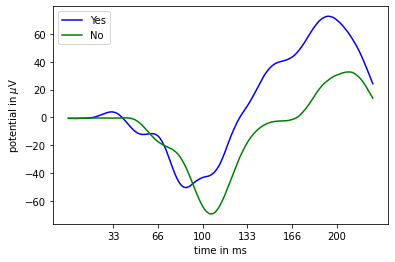
\includegraphics[width=0.50\linewidth]{images/thesis_fig3_3.png}
    
\caption{\label{experiment}\textbf{Experimental paradigm} \small The two different conditions are plotted for the tactile stimulus experiment. The 'Yes' (threshold) condition is defined in a way that 50\% of the stimuli were detected, whereas the 'No' condition is defined such that no stimuli were detected.}
  

\end{figure}

\subsection{Experimental paradigm}

In order to test how our pipeline can contribute to the study of an experimental or clinical paradigm, we used real ERP data, provided by \cite{jones2007neural}. This ERP data was source-localized to the somatosensory cortex and measured for two different conditions. In the first condition, a perceptual, tactile stimulus was detected in 50\% of the cases ('Yes'/threshold condition), whereas in the second condition, the stimulus was never detected ('No' condition). The stimuli consisted of brief taps of 100 Hz sine waves that were delivered to the hand \citep{jones2007neural}.
The difference of the waveform in the ERPs of the two conditions is visualized in Fig.\ref{experiment}. In a tutorial by the Jones Neurolab$^{\ref{tut}}$, the ERP waveforms coming from different conditions were fitted by the COBYLA algorithm. The algorithm adapts parameter choices by repeating optimization rounds that reduce the overall RMSE between the fitted and the real data. 
With this approach, one arrives only at a single point solution for each parameter. Besides, it does not allow for uncertainty measures. SBI, instead, allows to investigate the possibly vast or narrow solution space of the parameters.  \\
We test how SBI, in particular NIPE, is capable of finding differences in micro-scale processes between these two conditions. The marginals of the posteriors of the two conditions are compared with contour plots of the parameter densities that show the 68\% and the 95\% percentiles, which means that the area, where 68\% and 95\% of the posterior samples lay, is visualized.
We further show posterior predictive checks in order to see how the posteriors are able to recover the observations and how confident the simulated predictions are.
Beyond, we compare to the optimized values that were derived by the Jones Neurolab$^{\ref{tut}}$.








\chapter{Results}

\section{Gaussian toy example}


\subsection{Less simulations needed with NIPE, compared to SNPE}

\subsubsection{KL divergence}
\label{sec:results_kl}
The KL divergence is indicative for the quality of inference. The lower the KL divergence, the closer are inferred and analytic posterior. 
Fig.\ref{kldiv2} shows the comparison of the KL divergences between the inferred posteriors and the analytic posterior, with an increasing number of simulations per round. Inference was repeated 5 times for each method and for each number of simulations.

% Due to an instability issue when using mdn's with SNPE (issue \#669\footnote{https://github.com/mackelab/sbi}), we could not use the standard SNPE pipeline with mdn's where simulations of previous rounds are taken into account for calculating the new loss. 
% In order to test the performance with the standard SNPE pipeline with the \texttt{proposal= proposal} argument being set, 
 The variance of the KL divergence for SNPE is higher, indicating that inference was less steady and varied more between the 5 inferred posteriors compared to NIPE. Further, the mean KL divergence is lower for NIPE for all numbers of simulations.
 
 A masked autoregressive flow \citep{papamakarios2017masked} was used here.


\begin{figure}
 \centering
    % \begin{minipage}[h]{13cm}
    %     \small (a)  \hspace{6cm}  (b)  
    % \end{minipage}
        %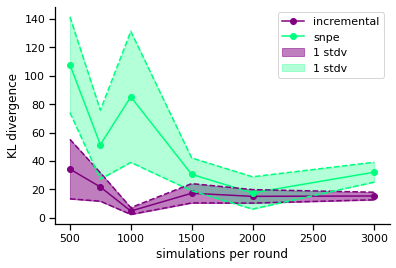
\includegraphics[width=0.42\linewidth]{images/thesis_fig4_3a.png}
        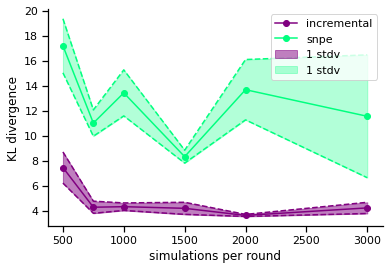
\includegraphics[width=0.5\linewidth]{images/thesis_fig4_1.png}
        %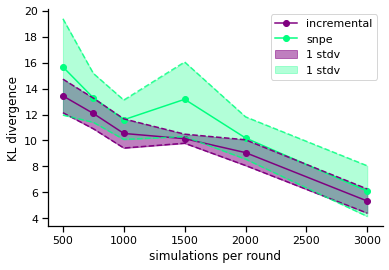
\includegraphics[width=0.31\linewidth]{images/thesis_fig4_3c.png}

        
\caption{\label{kldiv2}\textbf{KL divergence} \small for the SNPE approach (green) and the NIPE approach (purple). For each number of simulations per round, posteriors were calculated 5 times. The solid line describes the mean of the KL divergence between the 5 inferred posteriors and the analytic posterior. (a) inference with mdn. (b) inference with maf. }

\end{figure}


% \begin{figure}
%  \centering

% (a)
%         \includegraphics[width=0.4\linewidth]{images/sbc_incremental.png}
% (b)
%         \includegraphics[width=0.4\linewidth]{images/sbc_snpe.png}\\
        
% (c)
%         \includegraphics[width=0.31\linewidth]{images/cdf_incremental.png}
% (d)
%         \includegraphics[width=0.31\linewidth]{images/cdf_snpe.png}  \\
        

        
% \begin{tabular}{ c | c | }
%  \small \textbf{metric} & \ \small \textbf{NIPE}  \\ 
%  c2st ranks & \small .49 .53 .51 .51 .54 .51 .51 .59 .51 .52
%  .70 .61  .65 .60  .63  \\  
%  c2st dap & \small .49 .53 .51 .51 .54 .51 .51 .59 .51 .52
%  .70 .61 .65 .60 .63 \\
%  \textbf{metric} & \small \textbf{SNPE}  \\ 
%  c2st ranks & \small .50 .58 .52 .54 .52 .56 .53 .55 .57 .59
%  .65 .58 .56 .59 .56 \\
%  c2st dap & \small .47 .52 .50 .49 .48 .50 .50 .47 .47 .5 .51 .50 .48 .51 .50
% \end{tabular}

% (e)
        
        
% \caption{\label{sbc}\textbf{Simulation-based calibration} \small (a) Rank histograms for NIPE approach. (b) rank histograms for multi-round SNPE. (c) cumulative density function (cdf) of ranks with respect to the 95\% confidence interval of a uniform distribution (grey) for NIPE. (d) cdf for SNPE. (e) metric checks.}

% \end{figure}


\subsection{Reallocating simulation budget partially resolves over-dispersion of posterior}
\label{subsec:cal}

In order to check if the variances of the posteriors are under- or overestimated, we looked at the variances of the 15 single Gaussians, inferred with a maf as in the previous section \ref{sec:results_kl}. The variances are plotted in Fig.\ref{boxplot}, with box plots visualizing the distribution of the variances for the 5 repeated posteriors. We compare between NIPE and SNPE, and further between NIPE with equal simulation budget (lightblue) for the 3 steps and NIPE with reallocated budget (purple). A simulation budget of $\frac{1}{30}$ for the first step and accordingly $\frac{59}{30}$ is used for the last step for the NIPE variant with reallocated budget that we call 'NIPE-BUDGET' here.  \\


\begin{figure}[h]

%     \begin{minipage}[h]{12cm}
% \small (a)
%     \end{minipage}
 \centering
        %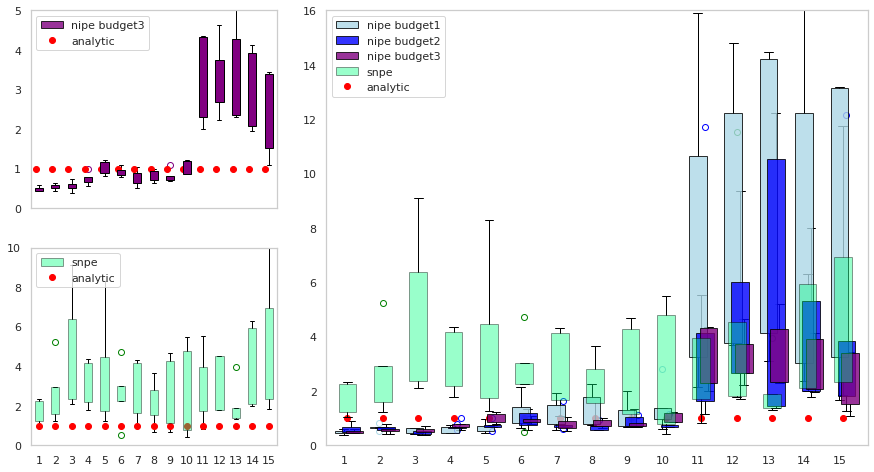
\includegraphics[width=0.99\linewidth]{images/thesis_fig4_4_boxplots.png}
        %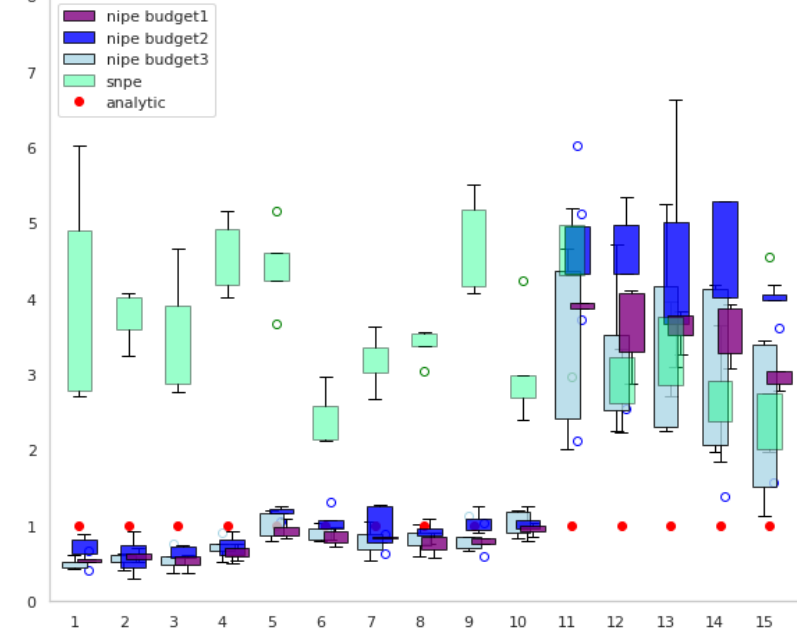
\includegraphics[width=0.7\linewidth]{images/box_plot_snpe_nipe_maf_budgets2.png}
        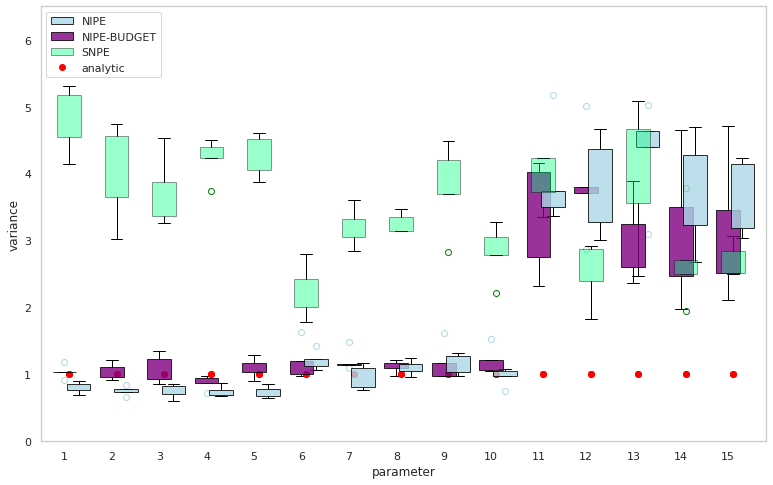
\includegraphics[width=0.8\linewidth]{images/toy_example_maf_03_05_ratio_notebook.png}
        
        
        
%     \begin{minipage}[h]{12cm}
% \small (b)
%     \end{minipage}
%         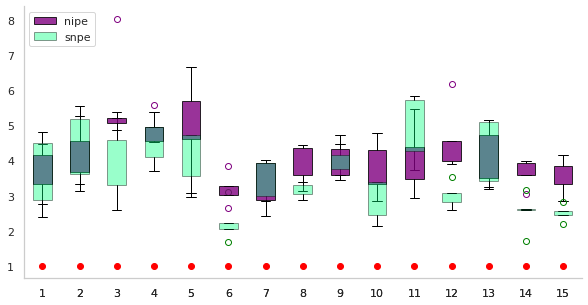
\includegraphics[width=0.7\linewidth]{images/box_plot_maf_not_restricted_further.png}
        
        
\caption{\label{boxplot}\textbf{Box plot for the variances of inferred and analytic posteriors} \small Visualizes the distribution (over 5 repetitions) of inferred and analytic variances of the posteriors. The red points describe the ground truth (std of 1) for the analytic posterior. The light green box plots show the distribution for the SNPE approach for every single parameter. The purple box plots show the variance distribution for the NIPE approach with reallocated budget, such that the last step gets more simulations (NIPE-BUDGET). The light blue boxes show the variances for NIPE with equal budgets in each step. }

\end{figure}

\textbf{NIPE}. For the Gaussians that were grouped into the first subsets, the variances for NIPE were slightly lower than the analytic variance, but well estimated for NIPE-BUDGET, with low dispersion between repetitions. The variances for the second subset are well estimated for both NIPE and NIPE-BUDGET. For the last subset, variances were higher than the true variance, and showed a wider dispersion between repetitions. The variances were a bit lower for the NIPE-BUDGET variant, but showed high dispersion between repetitions. \\

\textbf{SNPE}. The variances for the SNPE approach were for all parameters higher compared to the analytic variance, with a mean laying roughly between 2 and 5, with a moderate to high dispersion between repetitions. Further, sampling from the SNPE posterior took a longer time, with a sampling acceptance rate of roughly 0.124 percent if 1000 simulations were simulated in each round. The acceptance rate was even lower if a higher number of simulations were simulated per round. NIPE, in contrast, always had a sampling acceptance rate of 1.\\

In total, variances for NIPE were much lower compared to SNPE for the first two subsets, but showed a similar over-dispersion for the last subset. As the results seemed to improve a bit with NIPE-BUDGET, we used reallocation of budgets for for all further experiments.\\




\section{Event-related potentials}

Before we tested our pipeline on real data, we conditioned the posterior on a 'fake' observation that was simulated by the HNN simulator from a given parameter set that we define as the ground truth. This has the advantage that we can later compare the posterior marginals to the ground truth. In the following section, we start by comparing SNPE and NIPE on the basis of this simulated 'fake' observation. Later, we go on to test our approach on real data from the experimental setting that we have described in the methods section. 


\subsection{Summary statistic values are more restricted for the posterior, compared to the proposal distribution}

Checking the histograms of the summary statistics of the posterior and proposal, we can see that the histogram distribution of the summary statistics from the prior is much wider, as expected (Fig.\ref{histo1}). The true summary statistics are plotted in red. They are calculated from a 'fake observation' that has been simulated from parameters that are seen as the 'ground truth'. For all of the summary statistics, we can observe that the values derived from the posterior (in blue) are close to the true value. The values that are derived from the proposal are plotted in orange. Only 4 examples are plotted in Fig.\ref{histo1}. For all histogram plots, see the appendix \ref{histo_appendix}. .


\begin{figure}[h]
 \centering

        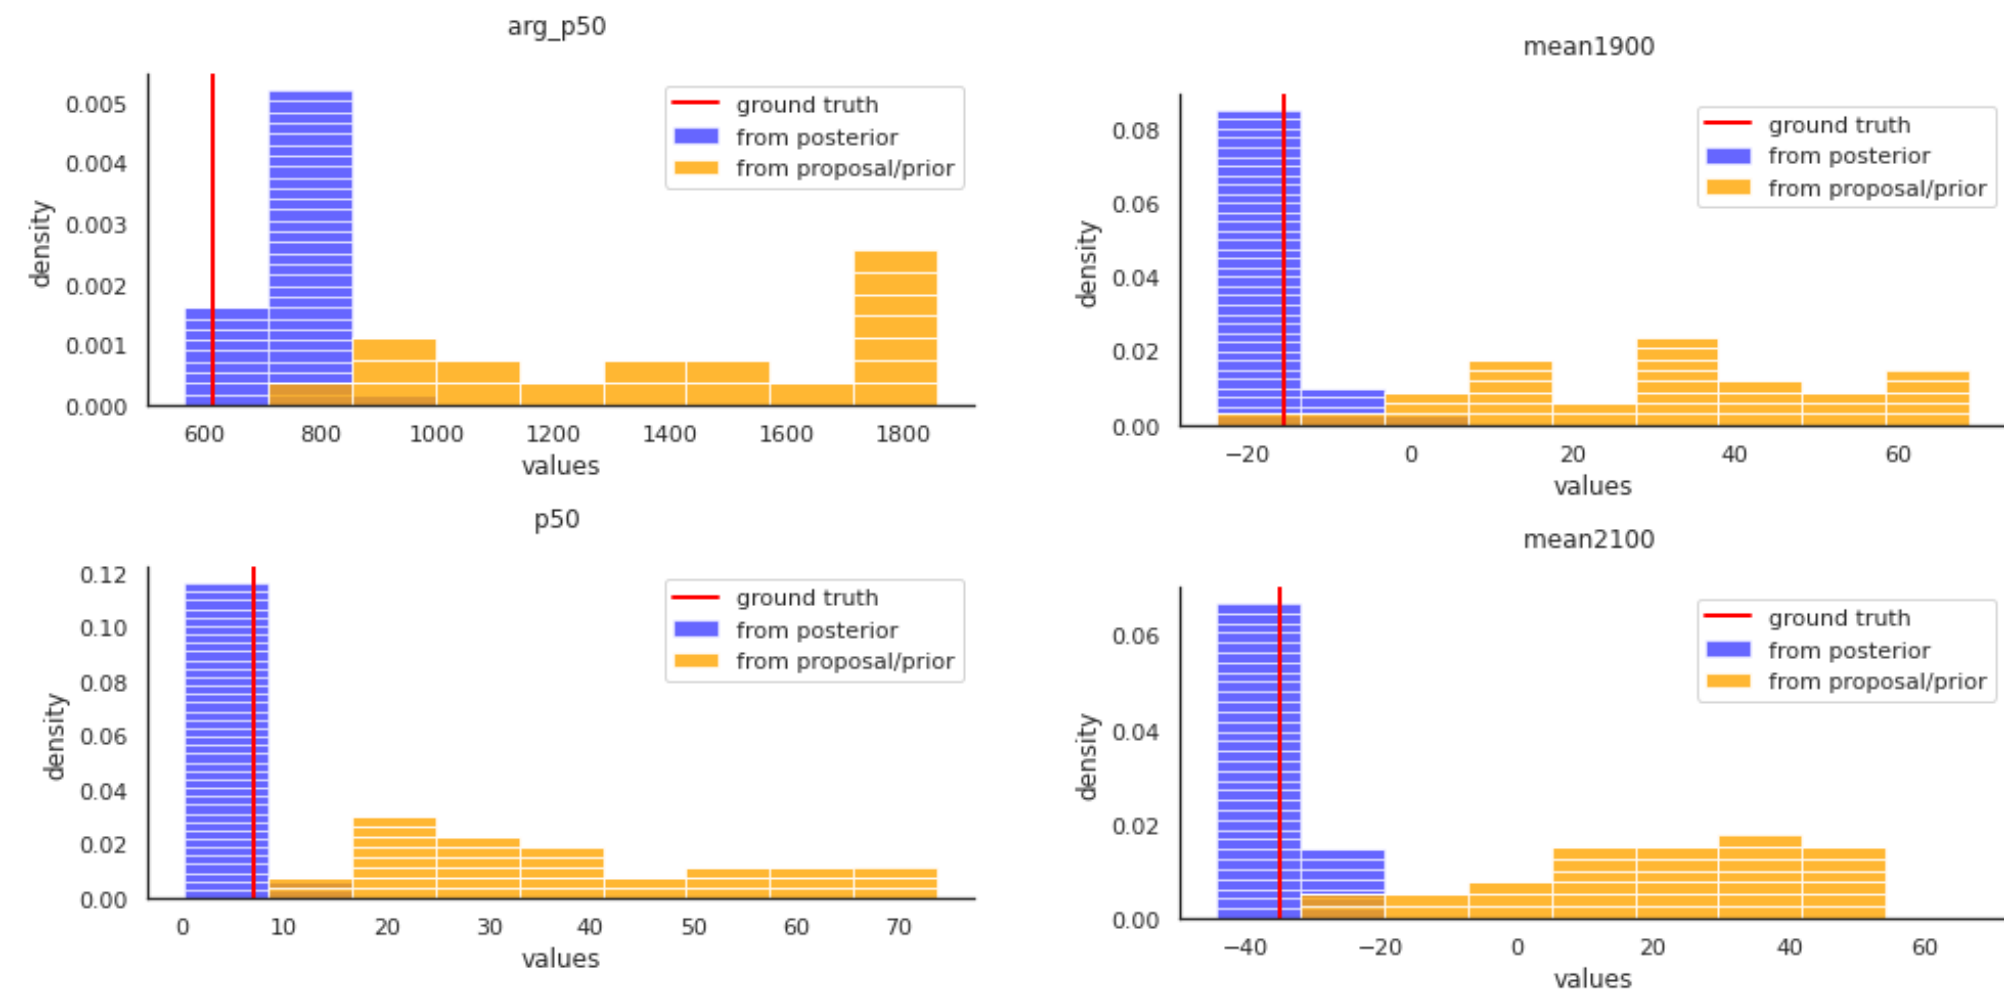
\includegraphics[width=0.99\linewidth]{images/histo_selection2.png}
        
        
\caption{\label{histo1}\textbf{Histograms for summary statistics} \small The histograms for the following four summary statistics are shown as an example: 'P50' describes the mean around the P50 component (10 ms before to 10 ms after the peak), 'arg\_p50' describes the time point of P50, 'mean1900' and 'mean2100' describe the mean for two particular time ranges. The values that are calculated from the prior samples are visualized in orange, while the values that are calculated from the posterior samples are visualized in blue. The red line indicates the ground truth. In this case, the ground truth is calculated from a 'fake observation' where we know the ground truth parameters and simulate this 'fake observation' from these ground truth parameters.}

\end{figure}

\subsection{Compensation mechanisms can be recovered by NIPE and SNPE } 



\textbf{NIPE approach}. The density plots and correlation matrices for the NIPE approach are shown in Fig.\ref{dens17nipe}. Total simulation and inference time was about 27 hours. Inference time was under a minute for the first step, around 13 minutes for the second step and around 24 minutes for the last step. The posterior was derived with a neural spline flow \citep{durkan2019neural} and a simulation budget of a $\frac{1}{7}$ was used for the first step and a $\frac{13}{7}$ for the last step (See \ref{sec:ratio}). 

The true parameters, plotted in red, mostly lay within the high density regions of the posteriors with some exceptions where the true parameters lay close to the high density regions, but not within. This was e.g. the case for the AMPA weights of L5 basket cells belonging to the first proximal drive and for the NMDA weights of pyramidal cells belonging to the distal drive. The shapes of the 2D marginals in the density plot and the correlation matrices indicate relationships between the parameters. There seem to be more correlations within the parameter subsets belonging to the same drive, and less between the different subsets. 

A positive correlation between the NMDA weights of L5 pyramidal cells and the onset of the first proximal drive is indicated in Fig.\ref{dens17nipe}a\&b. The same NMDA weights are negatively correlated with the onset of the distal drive. The onset of the first proximal drive and the onset of the distal drive are also negatively correlated.

A negative conditional correlation between the AMPA weights of L5 pyramidal cells and NMDA L5 pyramidal cells, belonging to the second proximal drive, is indicated in all plots of Fig.\ref{dens17nipe}. There is also a negative correlation between the NMDA weights of L2 and L5 cells belonging to the second proximal drive. In general, lots of parameters belonging to the second proximal drive are negatively correlated with each other.

Further, a negative correlation between NMDA weights of L5 pyramidal cells and the onset of the distal drive can be observed in all of the plots in Fig.\ref{dens17nipe}.

Interestingly, most of the weights belonging to the first proximal drive have multiple modes. There seem to be no conditional correlations between the weights of the first proximal drive, which could be related to the complicated shape of the marginals.

Looking at the posterior predictive checks in Fig.\ref{ppc_nipe_snpe}a, one can observe, that the 'true observation', plotted in red, is perfectly covered by the posterior area. The posterior area is more restricted for the early time range up to about 60ms, and then gets a bit broader. The 95\% confidence area of the posterior is sometimes not fully within the 95\% confidence area of the prior. \\

 \begin{figure}
 \centering


    \begin{minipage}{15cm}
        \small (a)  
    \end{minipage}
        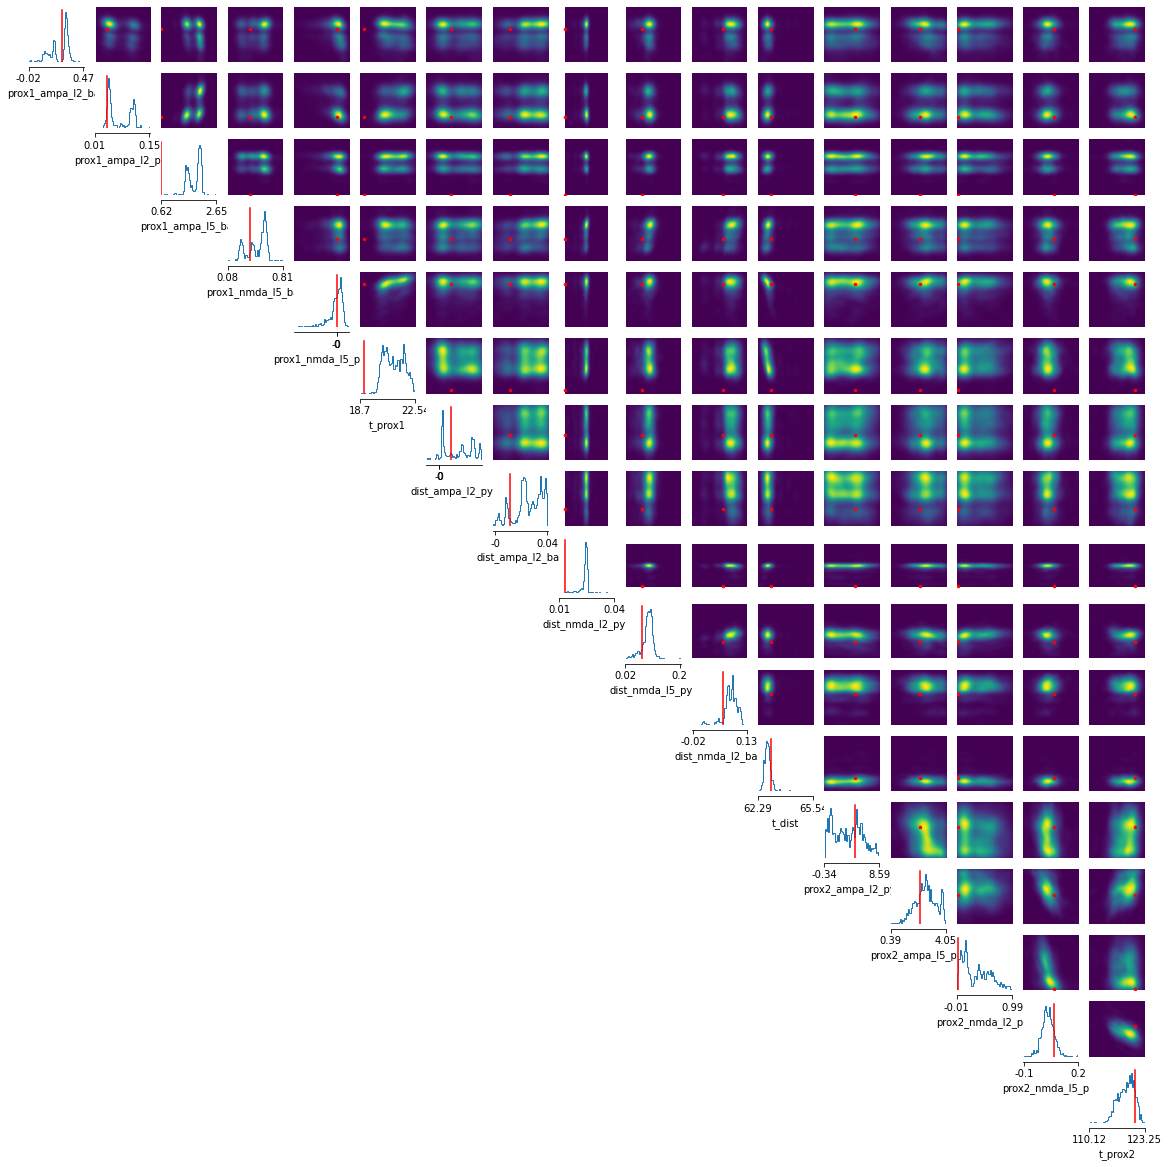
\includegraphics[width=0.92\linewidth]{images/thesis_fig4_6a_nipe.png}
    \begin{minipage}{13cm}
        \small (b)  \hspace{6cm} \small (c)
    \end{minipage}  
        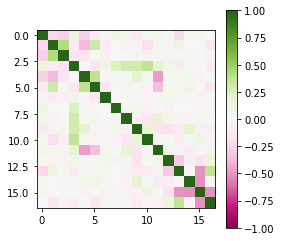
\includegraphics[width=0.37\linewidth]{images/thesis_fig4_6b_nipe.png}
        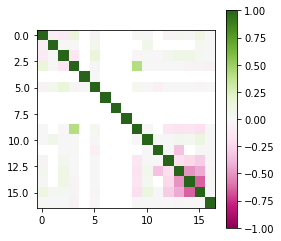
\includegraphics[width=0.37\linewidth]{images/thesis_fig4_6c_nipe.png}

        

\caption{\label{dens17nipe}\textbf{Density plots} \small Inference on 17 parameters with the NIPE method, using a neural spline flow. (a) density plot: 1D marginals are shown on the diagonal, whereas 2D marginals are shown off-diagonal, true parameters are plotted in red. (b) correlation matrix for the parameters. (c) conditional correlation matrix. }

\end{figure}


\begin{figure}
 \centering

    \begin{minipage}{12cm}
        \small (a)  \hspace{5.5cm} \small (b)
    \end{minipage}
        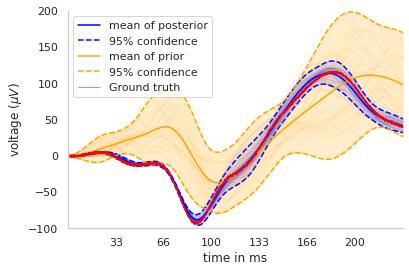
\includegraphics[width=0.4\linewidth]{images/thesis_fig4_7a.png}
        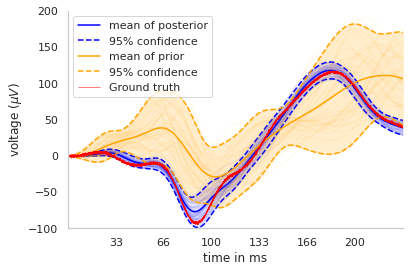
\includegraphics[width=0.4\linewidth]{images/thesis_fig4_7b.png}


        

\caption{\label{ppc_nipe_snpe}\textbf{PPC} \small Posterior predictive checks. The orange area describes the 95\% confidence interval area for the simulations from the prior. The blue area shows the same for the simulations from the posterior. (a) PPC for the NIPE approach. (b) PPC for the SNPE approach. }

\end{figure}


\textbf{SNPE approach}. Total simulation and inference time was about 40 hours. Inference time was 5 minutes for the first step, around 16 minutes for the second step and around 39 minutes for the last step.
The density plots for the posteriors derived with SNPE are plotted in Fig.\ref{dens17multi}. The true parameters are all laying in sampling regions of the posterior. The density plot indicates a negative correlation between the first proximal drive and the onset of the distal drive. According to the density plot, a later onset of the proximal drive would therefore correlate with an earlier onset of the distal drive. Further, the high density area of the 2D marginal between the AMPA weights of L5 pyramidal cells and AMPA weights of L2 pyramidal cells has a banana-like shape. According to the shape, a higher AMPA weight in L2 pyramidal cells corresponds to a lower AMPA weight in L5 pyramidal cells. 
The (conditional) correlation matrices indicate strong positive correlations between some parameters belonging to the first proximal drive, and some  strong negative correlations between parameters belonging to the second proximal drive. This is similar to the results for NIPE, except that there were no positive correlations between parameters of the first proximal drive indicated for NIPE. Besides, the 1D marginals for SNPE do not have multiple modes.

The posterior predictive check (Fig. \ref{ppc_nipe_snpe}b), shows that the 'true observation', plotted in red, is again perfectly covered by the posterior area. The posterior simulations are sometimes laying outside the area that is spanned by the 95\% confidence interval of the 100 prior simulations. Concerning the negative trough of the 'ground truth' signal, the confidence range for NIPE seems narrower, whereas the confidence range afterwards seems to be similarly broad for both approaches.\\


 \begin{figure}
 \centering

    \begin{minipage}{15cm}
        \small (a)  
    \end{minipage}
        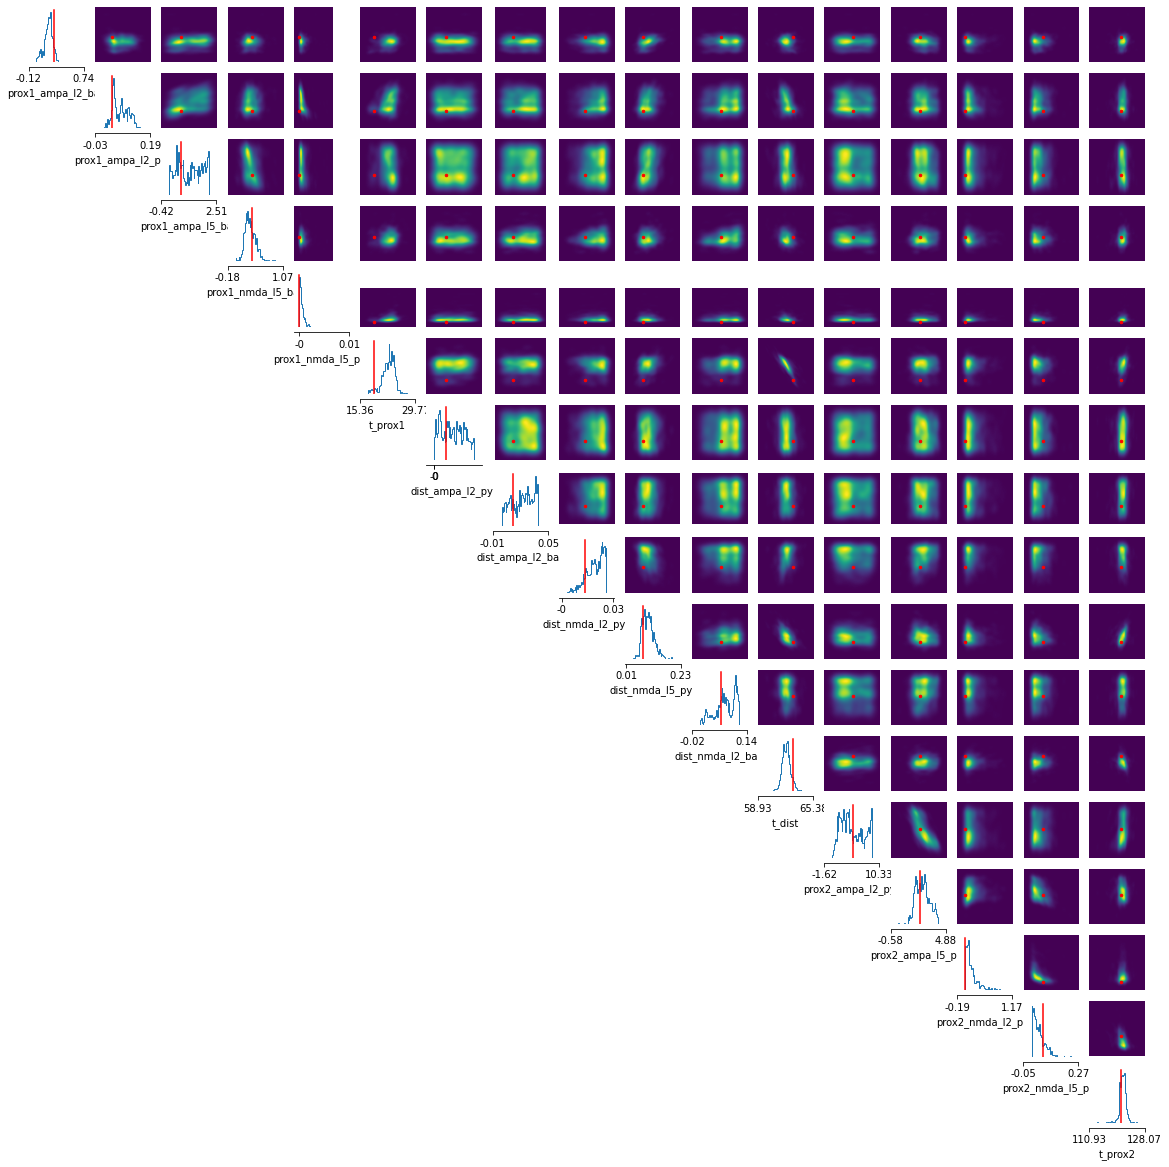
\includegraphics[width=0.92\linewidth]{images/kde_1000sims.png}
        
    \begin{minipage}{13cm}
        \small (b)  \hspace{6cm} \small (c)
    \end{minipage}  
        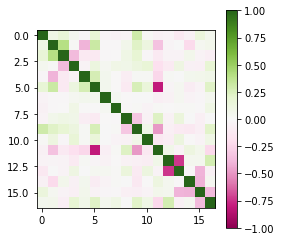
\includegraphics[width=0.37\linewidth]{images/thesis_fig4_8b.png}
        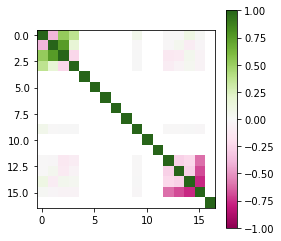
\includegraphics[width=0.37\linewidth]{images/thesis_fig4_8c.png}


\caption{\label{dens17multi}\textbf{Density plots} \small (a) density plot for SNPE (using a nsf density estimator). True parameters are plotted in red. 1D marginals are on the diagonal, while 2D marginals are off-diagonal. (b) correlation matrix. (c) conditional correlation matrix }

\end{figure}

\textbf{Comparison between SNPE and NIPE}. In order to evaluate differences in the inference process in one single plot, we plotted the 2D marginals of the NIPE approach in purple contours with 68\% and 95\% contour levels (Fig.\ref{contour_nipe_snpe}). The 2D marginals of the SNPE approach are plotted in green. This allows to investigate how the contours for the SNPE and the NIPE approach differ and how the parameter space within one single dimension gets restricted.  

The parameters of the first two subsets are restricted to a higher degree for NIPE, in comparison to SNPE. While for SNPE the true parameters always lay within the contour plots, for NIPE there are some exceptions. The parameters of the last subset are restricted a bit more by SNPE. \\

While drawing 1000 samples from the posterior took less than a second for the posterior inferred with NIPE, it took a long time for SNPE with an acceptance rate of only around 2e$^{-05}$. If prior ranges were expanded, the acceptance rate got even worse, such that sampling became unfeasible. We investigated whether this was due to a leakage issue such that most of the samples where not within the prior. Therefore, we plotted the densities for all samples, taking into account also the samples that were laying outside the prior support. The result of this can be found in the appendix (Fig.\ref{app_leakage}). Plotting the densities without excluding the samples laying outside the prior support revealed that the leakage was mainly due to negative values for parameter weights. Some symmetry between the 2D marginals for positive values and negative values could be observed (Fig.\ref{app_leakage}). \\

While total time for SNPE was around 40 hours, it took around 27 hours for both NIPE and NIPE-BUDGET(Fig.\ref{time}a). The results shown above are all derived by NIPE-BUDGET.
Fig.\ref{time}b visualizes how many milliseconds of the time series were simulated for each step/round. While for NIPE only 70 ms were simulated for the first step, for SNPE we needed to simulate the whole time series of 200 ms in each round. The differences are similar for CPU and simulation time, such that it seems likely that the main time difference between SNPE and NIPE was due to early stopping.\\

To recap shortly, the true parameters were better captured by SNPE, even though the posterior predictive checks seemed qualitatively equal for both approaches. Simulation time and sampling time was longer for SNPE. 

 \begin{figure}

    \begin{minipage}{13cm}
        \small (a)  \hspace{6cm} \small (b)
    \end{minipage}
     \centering
        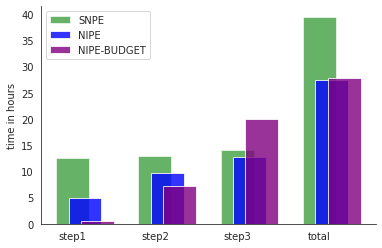
\includegraphics[width=0.41\linewidth]{images/thesis_fig4_9_time.png}
        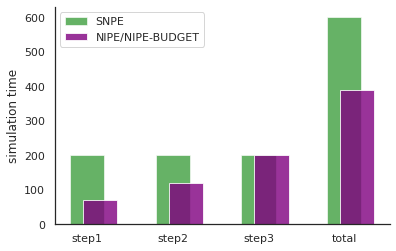
\includegraphics[width=0.41\linewidth]{images/thesis_fig4_9_simtime.png}



\caption{\label{time}\textbf{Time for each step - comparison between SNPE and NIPE} \small (a) The plot compares how many hours each step/round took for SNPE (green), for 'NIPE-BUDGET' (purple) and 'NIPE' (blue). The y-axis shows the time in hours (64 CPUs were used in parallel). (b) Plot visualizes how much time of the time series is plotted in each step/round. For NIPE, early stopping was used such that not the whole time series was simulated for the first two steps.}

\end{figure}

 \begin{figure}
 \centering


        %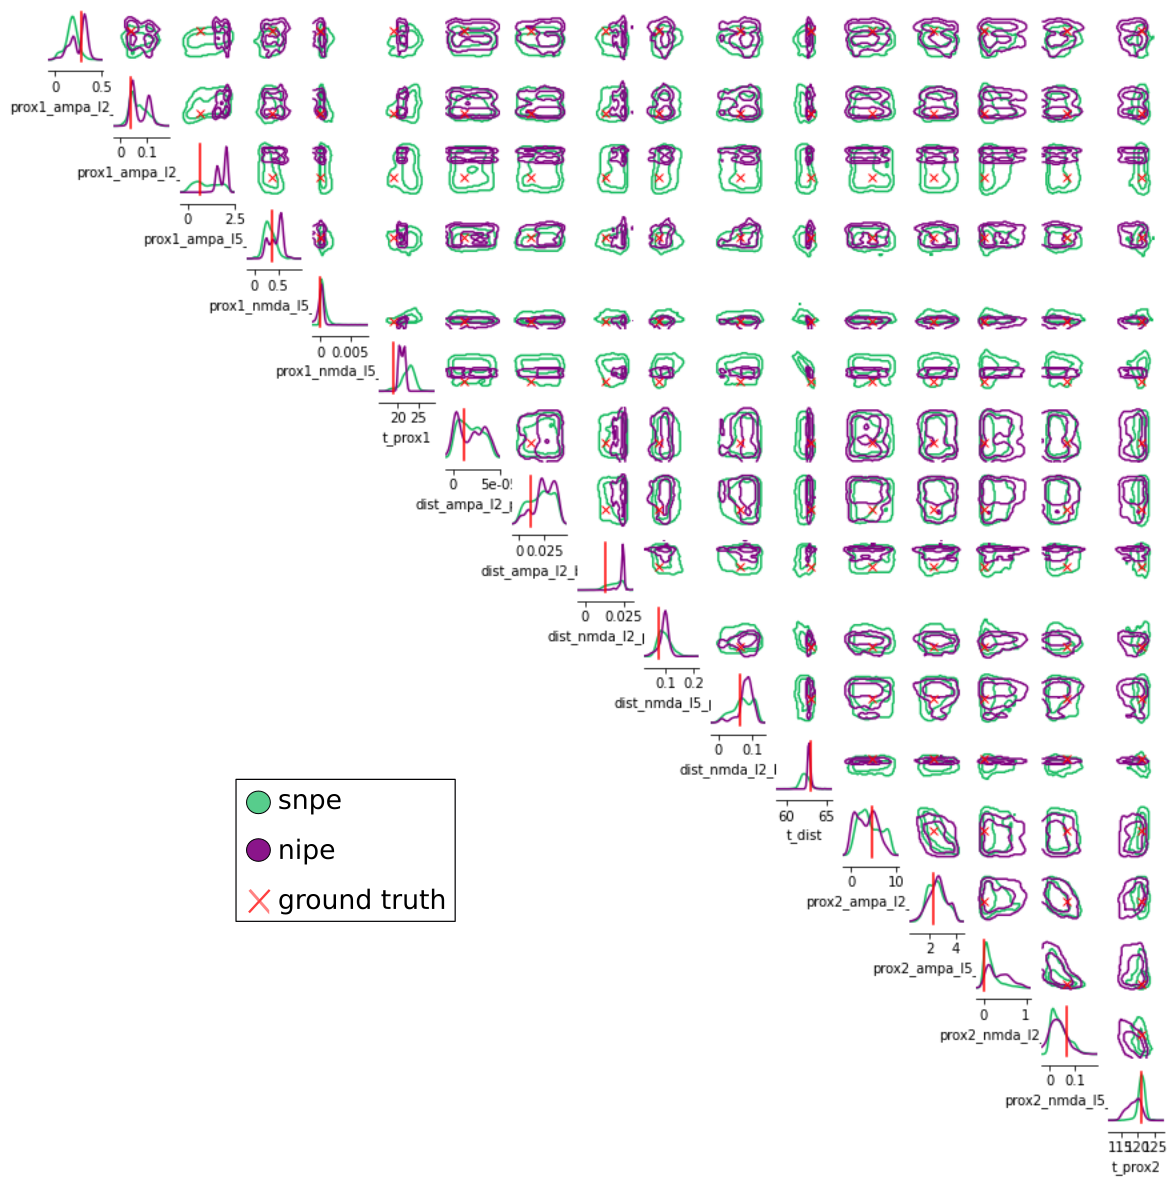
\includegraphics[width=0.99\linewidth]{images/thesis_fig4_10com_snpe_nipe_purple_green_label.png}
        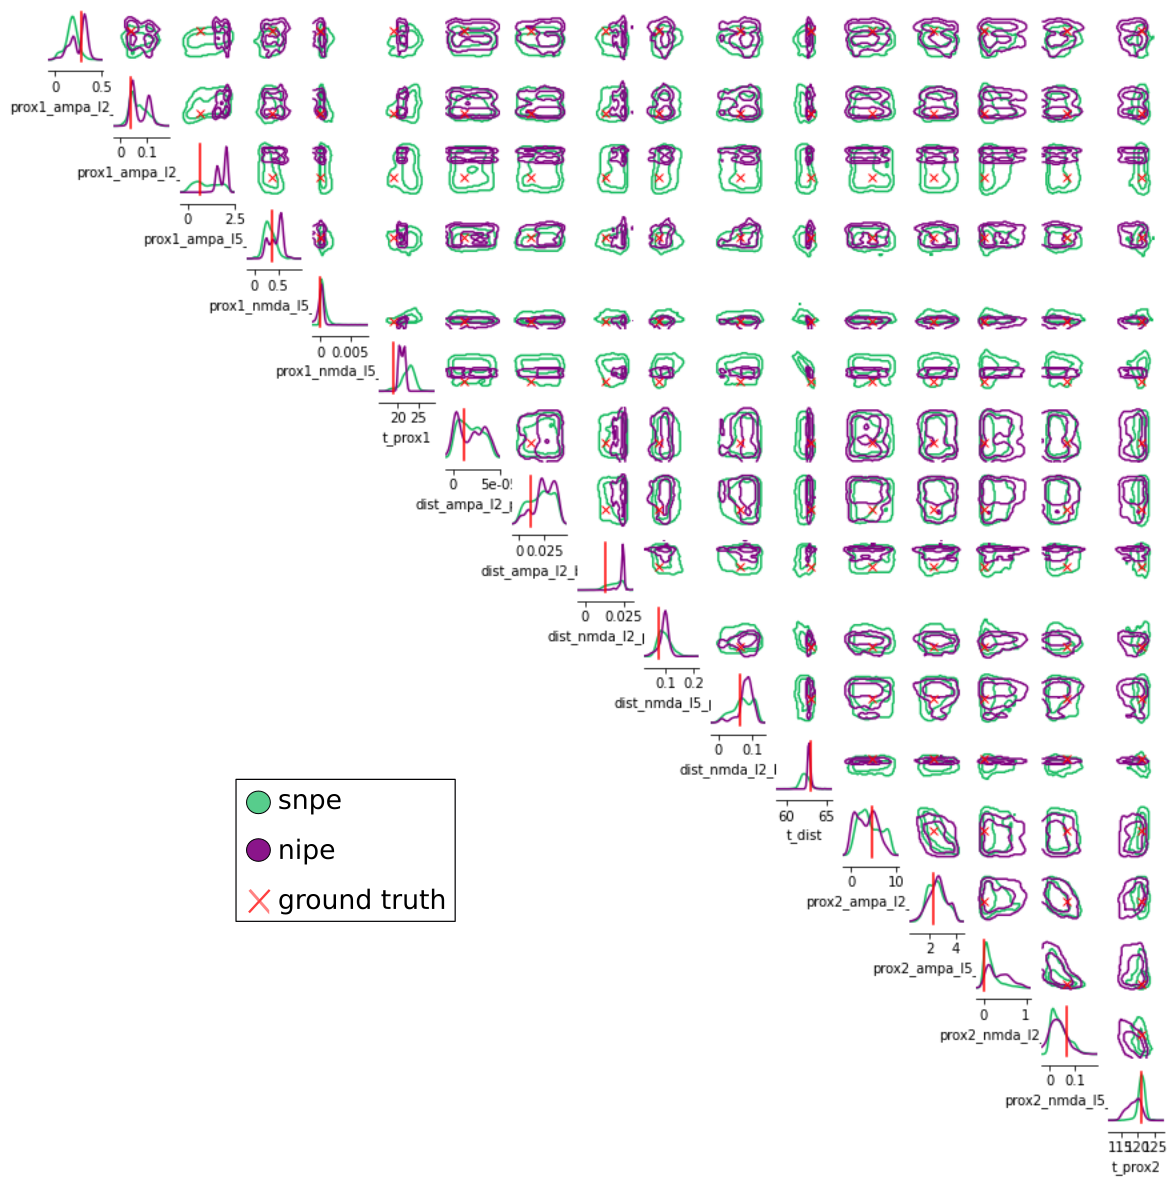
\includegraphics[width=0.99\linewidth]{images/thesis_fig4_10com_snpe_nipe_purple_green_label.png}


\caption{\label{contour_nipe_snpe}\textbf{Contour density plots - comparison between SNPE and NIPE} \small A nsf density estimator was used for both. 68\% and 95\% percentiles of the posterior densities are shown as contour lines. True parameter values are plotted in red. 1D marginals are on the diagonal, the 2D marginals off-diagonal. The results for SNPE are shown in green and the results for NIPE in purple.}

\end{figure}

\subsection{Parameter differences for the two conditions of the experimental paradigm}



\textbf{Posterior Predictive checks}. Fig \ref{exp_ppc} shows the posterior predictive checks for the conditions of the experimental paradigm. Plotted in blue, one can see the simulations sampled from the threshold posterior and plotted in green, the simulations are sampled from the 'No' posterior. The thick lines indicate the true observations on which the posteriors were conditioned on. We added some Gaussian noise to these. The single simulations are plotted in transparent colors. For each condition, 100 simulations were calculated. The areas that are bounded by the fine, dashed lines show the 95\% confidence intervals of the 100 simulations. In the threshold condition, there is a local maximum bump around 120 ms, whereas in the 'No' condition, the negative trough is prolonged and the P200 amplitude is lower compared to the threshold condition. 
The true observations are mostly covered by the 95\% confidence area of the 100 simulations drawn from each posterior. The posterior simulations are more restricted for the time range up to 100 ms and afterwards get a bit broader.


 \begin{figure}[!ht]
 \centering


        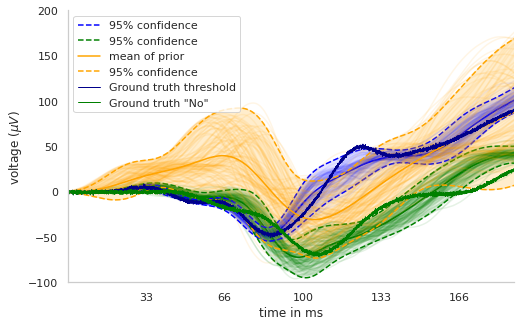
\includegraphics[width=0.70\linewidth]{images/ppc_threshold_versus_No_nipe.png}
        %(a)
        %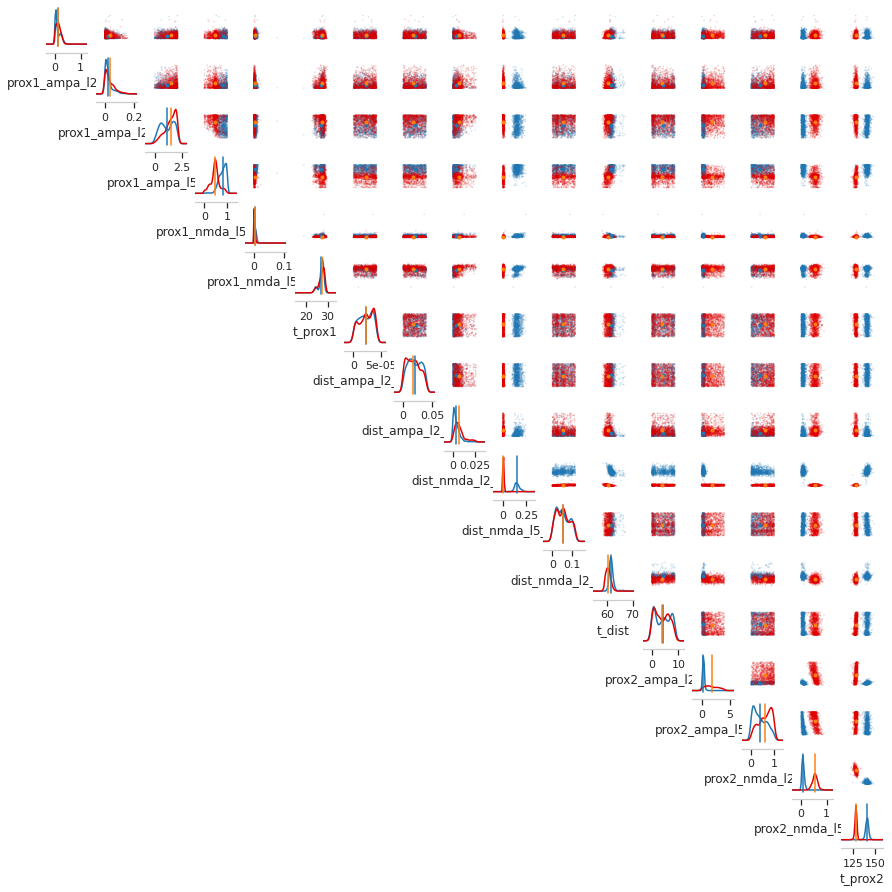
\includegraphics[width=0.45\linewidth]{images/scatter_density2.png}
        %(b)


\caption{\label{exp_ppc}\textbf{PPC - derived with NIPE (nsf)} \small The simulations drawn from the prior are visualized in orange (95\% confidence intervals), while simulations from the threshold samples are visualized in blue and simulations from the 'No' samples are visualized in green. The true observations are plotted in the same colors, but with strong, solid lines.}

\end{figure}


\textbf{Contour plots and comparison to the optimization values$^{\ref{tut}}$}. Fig.\ref{contour_opti} shows a contour plot of the 68\% and 95\% percentiles of the posterior densities for the two experimental conditions. In blue, one can see the densities for the threshold condition, whereas the densities for the 'No' condition are visualized in green. On the diagonal, one can see the 1D marginals, and the 2D marginals are plotted off-diagonal. 

We compared the inferred posteriors to the optimization values that were derived by the Jones Neurolab$^{\ref{tut}}$, plotting the 1D and 2D marginals of the posterior densities together with the point estimates derived by the Jones Neurolab. Fig.\ref{contour_opti} visualizes the densities for the threshold condition in blue, together with the point estimates that are plotted as blue lines and crosses. For the 'No' condition the point estimates are plotted as green lines and crosses.

The NMDA weights of L5 basket cells belonging to the first proximal drive are estimated to be higher by NIPE compared to the optimized values. There is a clear difference between the 1D marginals of the two conditions. The distribution for the 'No' condition is shifted to the left, such that values for the 'No' condition are estimated to be lower. The optimized values in contrast are estimated to be 0 for both conditions.

Whereas the optimized onset for the first proximal drive was estimated to be '26.61' for the threshold condition and '40.6' for the 'No' condition, the posteriors derived by NIPE lay close together, with the highest density laying a bit under '30'. 

The optimized values for the onset of the distal drive match well with the high density areas of the 2D marginals. The distal drive's onset of the 'No' condition is estimated to be later than the onset for the threshold condition.

The second proximal drive's onset is estimated to be later for the 'No' condition than for the threshold condition, both by NIPE and by the optimization. The posterior peaks are laying further away, even though the optimized values are still within the outer contour borders. The other weights belonging to the second proximal drive are stronger restricted for the 'No' condition, compared to the threshold condition.

In the tutorial, it was mentioned that 'changing the standard deviation was necessary for matching the minimum and spread of the experimental dipole data at 75 ms'$^{\ref{tut} }$. If we included the standard deviation as a parameter, however, our SBI pipeline did not work well anymore and was not able to predict observations from the posterior anymore. Posterior predictive checks also got worse when we widened the prior for the AMPA weights belonging to the distal drive. We widened them because the optimized values for the 'No' condition were not contained in our initially chosen prior range. Widening the prior seemed to favor simulations with a deep negative trough that did mostly not include the observation anymore. Hypothetically, the number of simulations did then not suffice anymore to restrict the posterior to a satisfactory degree. We therefore kept our initial prior, such that the optimized values were not included in our prior for these AMPA weights. For this reason, one cannot find the optimized values for these two parameters in Fig.\ref{contour_opti}.\\

To sum up, the contour plots visualized some differences of the 1D and 2D marginals between the two experimental conditions. The parameter values derived by the optimization$^{\ref{tut} }$ and the 1D marginals matched well for some parameters, but deviated a lot for others, as well. The posterior predictive checks suggest that the inferred posteriors were able to predict differences of the conditions.






 \begin{figure}[!ht]
 \centering


        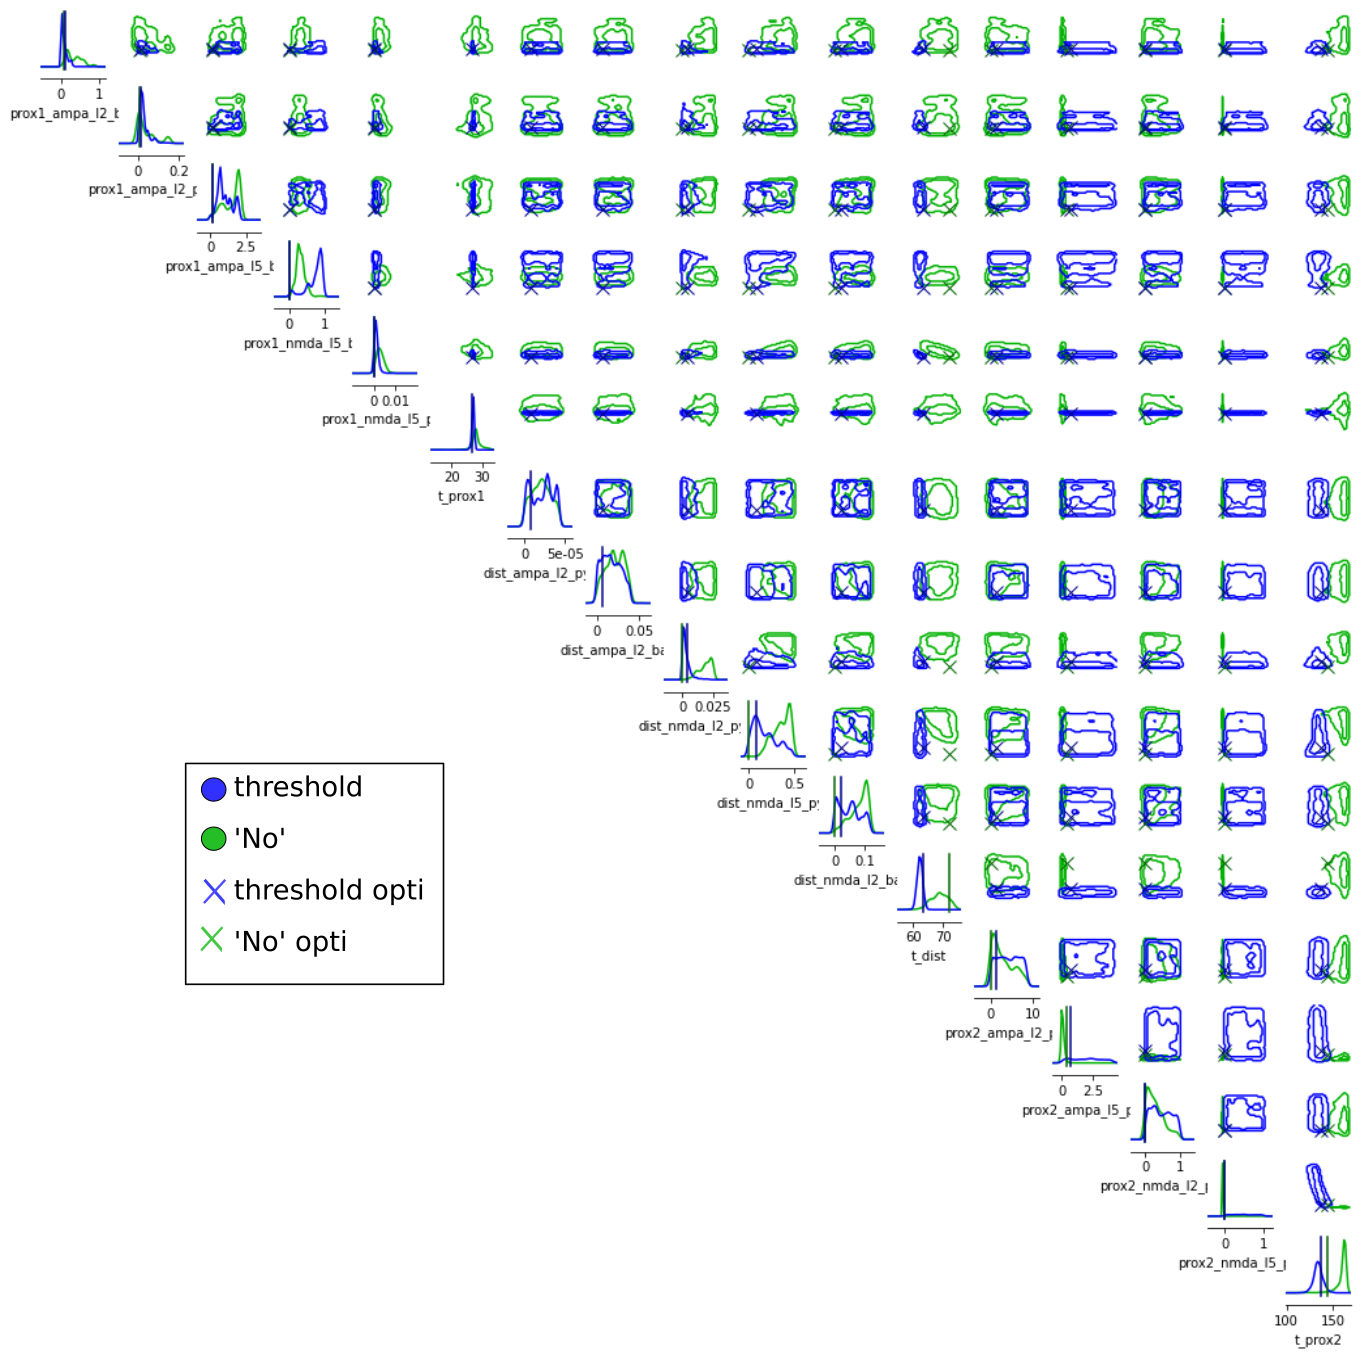
\includegraphics[width=0.99\linewidth]{images/contour_plots_threshold_versus_no_green_blue4.png}
        


\caption{\label{contour_opti}\textbf{Density plot - Comparison to optimization tutorial} \small (a) shows the 1D (diagonal) and 2D marginals (off-diagonal) for the threshold condition (blue) and the 'No' condition (green, derived with NIPE. The green crosses and lines indicate the optimized values of the 'No' condition from the tutorial, while the blue crosses/lines indicate the same for the threshold condition.}

\end{figure}











\chapter{Discussion}



%\subsubsection{Toy examples}
We showed that NIPE performs well with respect to the KL divergence and the quality of the density plots. Further, the results indicate that NIPE is more time- and sampling-efficient, compared to SNPE. The calibration check, however, revealed a bias regarding the estimated variances of the single parameter posteriors inferred by NIPE. Parameters that were inferred later in the inference pipeline showed a higher variance and were over-dispersed, while parameters that were inferred in the first step showed a bit of an under-dispersion. If we used NIPE-BUDGET as a variant, where we reallocated the simulation budget towards the last subset, we could reduce the issue of under- and over-dispersion to a certain degree, but did not resolve it completely. How posteriors can be well calibrated should be addressed in future research. Future research could investigate how to include simulations from former steps and importance weights, similarly to SNPE \citep{greenberg_automatic_2019}. Unfortunately, there is no straightforward way for NIPE because in each step we use a different number of parameters, such that it is not clear how to combine simulated parameter vectors of different length. 

Nonetheless, in a time-series setting where we assume time-dependencies of the parameter subsets, it is even realistic that parameter estimations for later subsets have a higher uncertainty because they depend on parameter estimations from earlier subsets. For the Gaussian toy example, there are no dependencies between parameters and therefore conclusions for time-series problems are limited.  \\



%\subsubsection{Summary statistics}

We were able to show that the designed summary statistics for ERPs restricted the prior space. It is difficult, however, to estimate the sufficiency of these summary statistics without knowing the ground truth posterior. If the ground truth is known, one could, e.g., calculate the KL divergence with and without a certain summary feature in order to see how and if the feature restricts the posterior. One could then add features, dependent on how they contribute to a lower KL divergence. Adding more summary statistics, makes inference more complex and slower, such that we have to limit the number of summary statistics to a reasonable amount. Finding the most contributing summary features was beyond the scope of this work and could be an interesting target for future research.\\


%\subsubsection{Validation checks and compensation mechanisms}
Regarding ERPs, we showed similar density plots with respect to density shapes and covering of the ground truth of the parameters for SNPE and NIPE. As we do not have experimentally derived ground truth parameters, the interpretation of inference quality is limited. Nevertheless, we can evaluate if the true parameters are being recovered by the posterior densities. This was the case for both approaches, even though the true parameters were to some extend better recovered by SNPE. The posterior predictive checks indicated that both methods could well recover the true observation. \\

Certain shapes in the 2D marginals of the posteriors indicated compensation mechanisms between parameters. Stronger AMPA weights of L5 pyramidal cells, belonging to the second proximal drive, can probably compensate for weaker NMDA weights of L5 pyramidal cells. Further, if the onset of the proximal drive is later in time, the distal drive has to start earlier for deriving a similar ERP curve. The correlation seems plausible because the distal drive as a counterpart for the proximal drive, has to exhibit its drives earlier on in order to push against the forces of the proximal drive. 

Another compensation mechanism was indicated between the AMPA weights in L2 pyramidal cells and the AMPA weights of L5 pyramidal cells, belonging to the second proximal drive. They correlate negatively, such that one of them can be increased if the other one is decreased in order to derive the same outcome. Both parameters correlate positively with an increased amplitude of the P200 component, also mentioned in the Jones tutorial$^{\ref{tut} }$. Increasing only one of them should suffice to increase the amplitude. One can also increase one parameter and decrease the other one for arriving at the same P200 amplitude again.
We verified these correlations by sampling from the default parameters and changing one of the two parameters at a time, while holding all other parameters fixed.

We observed a positive, conditional correlation between AMPA weights of the L2 pyramidal cells belonging to the first proximal drive and the ones belonging to the distal drive. If one of them increases, the other one has to be increased as well in order to derive the same result. Strong AMPA weights belonging to the distal drive might weaken the AMPA weights belonging to the first proximal drive, such that increasing both weights results in the same output.\\


Overall, we found some interesting compensation mechanisms that suggest that some parameters act as counterparts whereas others can act as amplifiers. Concerning the 'amplifiers' that seem to have the same function/mechanism, the question arises if the HNN model could be compressed such that e.g AMPA weights of L2 and L5 cells belonging to the same drive, could be combined in one single parameter.\\

% By studying compensation mechanisms, SBI has also the potential to contribute to the study of plasticity and self-organizing behavior. 
% \cite{effenberger2015self} e.g. study how homeostatic processes play a role in stable self-organization of the brain. Investigating correlations between mechanisms with SBI could help with understanding how plasticity and self-organizing behavior evolve in the brain. Compensatory mechanisms could teach us about plasticity, showing that different combinations of micro-scale processes might lead to the same macro-scale signal. As mentioned earlier on, \cite{marder2011multiple} argue that one should study the population of models instead of a single one. If we allow enough flexibility and stochasticity in our model, we probably achieve the same goal by studying the posterior densities of the model parameters with the SBI pipeline.\\

The contour plot comparison between NIPE and SNPE hinted at a possible bias insofar that parameters of earlier subsets seemed to be better restricted for NIPE in comparison to SNPE, while it was the
opposite for the last subset. The 1D marginals belonging to the first subset had a more complex shape, in comparison to SNPE. If this indicates under-dispersion or a better restriction of the parameter space, remains an open question. As both SNPE and NIPE are sequential methods, we can not apply simulation-based calibration. How and if simulation-based calibration could be made applicable for sequential methods, needs to be discovered in further research. When using NIPE, one has to be aware of possible biases of the posterior variance. If simulation budget is not an issue, SNPE might be the better choice.

Sampling from SNPE posteriors, on the other hand, was often very slow. We showed that this was due to a big sampling leakage such that most of the samples were outside the prior support. If efficient sampling is needed, NIPE has a huge advantage over SNPE as it does not suffer from this sampling issue. Especially when wider prior ranges were chosen, sampling from SNPE was not feasible anymore. This is a well-known problem for SNPE, when using maf or nsf estimators. It could help to project the parameter samples to an unbounded space for inference and afterwards project the posterior samples back to constrained space again, as explained by \cite{gonccalves2020training}. In order to make multi-round SNPE more sampling-efficient, this could be interesting to investigate in further research. \\

%\subsubsection{Stochasticity, standard deviation}
In general, it is not an easy question which parameters to include in the inference process. It is for example disputable whether it is better to use a small subset of parameters that we want to investigate while leaving other parameters fixed, or instead use all available parameters of a model. The later makes inference a lot harder, the former possibly prevents the exploration of the whole parameter space. If one is only interested in compensation mechanisms of a small subset, it might not be necessary to include all parameters of the model, but one could carefully select the parameters of interest. 

Ensuring stochasticity of a simulator is a crucial part for SBI. This is because inference should be robust to small perturbations of the processes. There is evidence that there are many adaptive and compensatory mechanisms going on in the brain that can cope with perturbations \citep{marder2011multiple}. Inducing stochasticity into a simulator should therefore make inference robust, but at the same time make it more biologically realistic.

If adding observation noise and choosing \texttt{sigma}$>0$ is inducing an appropriate degree of stochasticity has to be tested in real experimental studies. To our knowledge, there does not exist experimental (animal) ERP studies that have tested mechanistic models like the HNN and proofed that the model predicts parameters well. The HNN model has been compared to animal studies in the case of beta bursts in the motor cortex, which is one of the best studied movement signals \citep{bonaiuto2021laminar}, but this has not be done for ERPs, yet.
We made the experience that, when including \texttt{sigma} as a parameter, inference was either not possible, or it took a long time and even then did not restrict the parameter space well. Hypothetically, including \texttt{sigma} as a parameter makes the model very flexible such that much more simulations would be needed for inference. Fine-tuning as in the Jones tutorial$^\ref{tut}$ might be possible, but does not seem appropriate for our case.  

%\subsubsection{Smoothing window}
We used a smoothing window of 30 ms for the time series, which might be too wide to capture interesting local bumps, but might make inference more robust. In the Jones optimization tutorial$^{\ref{tut}(Fig.11)}$, it is mentioned that compared to the threshold condition, the supra-threshold condition has very sharp features and therefore needs a shorter time window. We did not vary time windows for different conditions. This might have arguably improved our results. Nevertheless, this again is some form of fine-tuning that should optimally not be needed. \\




%\subsubsection{Experimental paradigm}

For the experimental paradigm, we observed mainly differences between the conditions for the onset of the distal drive and the onset of the second proximal drive. Some conductance weights were more restricted by one of the conditions, which implies that the weights might only play a role for a certain condition, while it does not get restricted a lot for another one. 

The posterior predictive checks indicated that the simulations from the posterior samples matched the observations well and the simulations from the two conditions were well differentiated. We could show that NIPE was able to restrict the parameter space and to differentiate the conditions via parameter posteriors.

Widening the prior ranges led to a lower restriction of the posterior for the 'No' condition, such that we kept our initial prior ranges. However, we did possibly not investigate the full solution space by restricting the prior range too much. Prior ranges should not vary for different conditions in order to not induce strong inductive biases. Finding appropriate priors that are able to find all biologically plausible mechanisms, is therefore an important task for further experiments. \\




%\subsubsection{Limitations}

\textbf{Further limitations.} Our approach is not amortized, such that a trained neural density network cannot be conditioned on new observations.
It could be very practical to make the approach amortizable, such that inference is less costly and time-consuming. Unfortunately, this is not straightforward for sequential approaches where the parameter space gets restricted by an observation after each round and is therefore conditioned on a particular observation. \\


NIPE is based on specific assumptions, e.g. that there exists a time order for parameter subsets such that earlier subsets of parameters have an effect on later subsets, but not the other way. This assumption makes it possible to separate the inference process in smaller parts where we have to deal with a much smaller dimensionality. The approach is limited to problems where we can make similar assumptions. Nevertheless, we think that this assumption is met by many problems that are investigated in neuroscience research as time series like EEGs or spike trains always have a natural time order. 
\cite{prangle2016lazy} introduced an approach where simulations of time series were interrupted if they did not seem promising. We, in contrast, used early stopping and showed that it reduced simulation time by a significant amount. Early stopping could be used in any problem were the above mentioned assumptions can be met, which could help in making SBI more affordable for problems with costly simulations.  \\

% Further, it would be interesting to not only condition on a single observation, but instead on many observations, belonging to the same condition. This would be very helpful for investigating clinical conditions where there might be a certain variance between e.g. patients with schizophrenia, but where one would like to investigate what the commonalities within a condition are. 


\section{Conclusion}

Overall, our approach offers an opportunity to investigate high-dimensional problems that usually need a huge amount of simulations with other methods often used for model-inversion of the brain like MCMC \citep{hashemi_bayesian_2020}. 
Further research should examine how NIPE can be better calibrated such that neither later inferred posteriors are over-dispersed, nor earlier inferred posteriors are under-dispersed.\\

We showed several compensation mechanisms that suggest that it is sometimes possible to increase one parameter and decrease another one, without changing the final output. Including more parameters increases the chance for degeneracy to occur. We also made the observation that including \texttt{sigma} as a parameter introduces too much flexibility, such that inference is not possible anymore or rather would have needed much more simulations. Whereas point estimates provide only one single solution, we visualized that there is a broader solution space. We therefore offer an approach that is able to show parameter uncertainties. \\

Applying NIPE on an experimental paradigm, interesting differences of the two conditions on the micro-level were shown. Revealing micro-scale differences between conditions can contribute to precision medicine applications by providing patient-specific suggestions that make clinical interventions more effective. Our method has the potential to fill the gap between micro- and macro-dimensions through studying the interaction of micro-processes and the emergence of complex macro-signals. It can be used to test hypotheses about biophysical processes and to discover medical treatment alternatives. \\

Their is evidence that the feed-forward and feedback information flow through the layers, and also the laminar structure, is shared across different sensory regions \citep{kohl_neural_2021, atencio2010columnar}. Applying SBI in combination with the HNN model, can therefore be applied for many different sensory tasks, e.g. tactile, auditory or visual tasks. This opens the door for different scientific questions and interesting clinical applications. 

In future experiments, it would be interesting to find experimental designs that test how well the biophysical model is specified. Here, we suppose that the assumptions made by the model are well justified and can reveal e.g. clinical or cognitive conditions. How these assumptions can be validated, however, remains an open research question.


\chapter*{Acknowledgments}
I want to thank Prof. Jakob Macke, who gave me the possibility to combine my interests in neuroscience and machine learning methods and who gave ideas, interesting paper proposals and feedback during the process of my thesis. I also want to thank Prof. Martin Butz, who volunteered to be my second supervisor. \\

My special thanks goes to Cornelius Schröder, who always gave new ideas, valuable feedback and time for asking questions. We were exploring lots of ideas and different directions and he gave great guidance on where to focus and how to approach various ideas. \\

In general, I want to thank the Macke group for their hospitality, valuable feedback and interesting discussions during lunch time and coffee breaks. 







\bibliographystyle{plainnat}
\bibliography{MyMasterThesis}



\chapter{Appendix}


\section{Toy example - Piecewise linear function}
\label{piecewise_sec}

\subsection{Method procedure}

To get a first impression how the NIPE approach performs, we tested it with a simple toy example - a piecewise linear function where one can vary offset and slope parameters. The model was defined with 3 pieces in the following way:

$$ y[x<cp_1] = b + a_1 \cdot x + \epsilon$$
$$ y[cp_2\leq x\leq cp_2] = y_{cp_1} + a_2 \cdot x +\epsilon$$
$$ y[x \geq cp_1] = y_{cp_2}  + a_3 \cdot x+ \epsilon$$

, where $a_1$: first slope, $b$: offset, $a_2$: second slope, $a_3$: third slope, $cp_1$ and $cp_2$: changing points, $\epsilon$: noise. $y_{cp_1}$ and $y_{cp_2}$ are the function values at the changing points.\\


We varied 4 parameters - the offset and the 3 slopes. The ground truth was arbitrarily set at the beginning. The posteriors were conditioned on the observation under the defined ground truth.  \\

For the NIPE approach, we defined 3 inference steps and set the number of simulations to 300 for each of these steps. In the first step, we simulated only the first piece up to $cp_1$, and then inferred the posteriors for $b$ and $a_1$. The posteriors for $b$ and $a_1$ were combined with the prior for $a_3$, such that parameters $b$ and $a_1$ were sampled from the posterior and parameters $a_2$ were sampled from the prior. In the second step, we then simulated up to $cp_2$ and inferred the posteriors for $b$, $a_1$ and $a_2$. For the third step, $a_3$ was inferred as well.

For the SNPE approach we used a multi-round approach (3 rounds) and used 300 simulations for each round. 

We then used posterior predictive checks  and density plots of the inferred posteriors to compare the two approaches. 

\subsection{NIPE restricts piecewise linear model to a higher extend}

Testing the NIPE approach on the piecewise linear toy example shows that it performed really well. With the same amount of simulations (900 in total), the NIPE approach makes equally good predictions, compared to SNPE, according to the posterior predictive check (Fig.\ref{piecewise}). It restricts the parameter space to a higher extend, which is observable from the density plot (Fig. \ref{piecewise2}).\\
The whole simulation and inference process took about 30 seconds for both approaches.



\begin{figure}
    \begin{minipage}{15cm}
        \small (a)  \hspace{4.3cm}  (b) \hspace{4.3cm}  (c)  
    \end{minipage}
 \centering

    \begin{subfigure}{.32\textwidth}
        \centering
        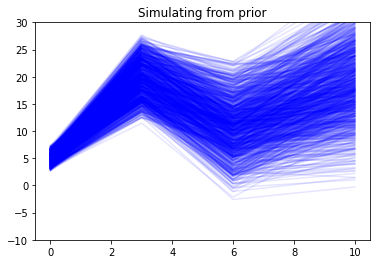
\includegraphics[width=1.\linewidth]{prior_piecewise.png}
    \end{subfigure}
    \begin{subfigure}{.32\textwidth}
        \centering
        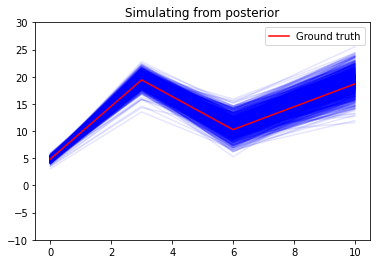
\includegraphics[width=1.\linewidth]{piecewise_ppc_snpe_final.png}
    \end{subfigure}
    \begin{subfigure}{.32\textwidth}
        \centering
        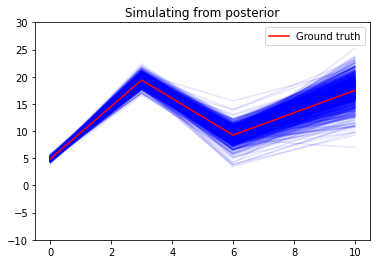
\includegraphics[width=1.\linewidth]{piecewise_ppc_incremental_final.png}
    \end{subfigure}
    
\caption{\label{piecewise}\textbf{Post-predictive checks: Piecewise linear model} \small (a) shows simulations from samples drawn from the prior. Inferring the parameters (slopes and changing points) with the SNPE approach (b) and the NIPE approach (c). The ground truth is plotted in red. The plot visualizes how the posteriors restrict the simulation space.}
  

\end{figure}


\begin{figure}[h]
    \begin{minipage}{10cm}
        \small (a)  \hspace{7cm}  (b)  
    \end{minipage}
    
     \centering

    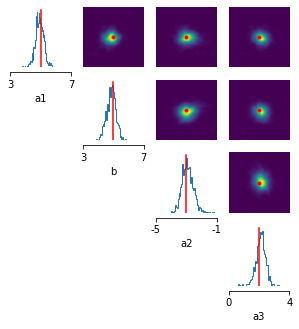
\includegraphics[width=0.45\linewidth]{piecewise_density_plot_snpe_final.png}
    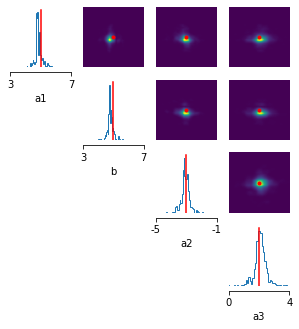
\includegraphics[width=0.45\linewidth]{piecewise_density_plot_incremental_final.png}



    
\caption{\label{piecewise2}\textbf{Piecewise linear model} \small Density plots for (a) the SNPE approach  (b) the NIPE approach. The 1D marginals of the posteriors are plotted on the diagonal, while the 2D marginals are shown off-diagonal. The red lines/points indicate the ground truth of the parameters. $a_1$ to $a_4$ are the slope parameters of a piecewise linear function while $b$ describes the offset.}
  

\end{figure}



% \begin{figure}[h!]
% \centering

% 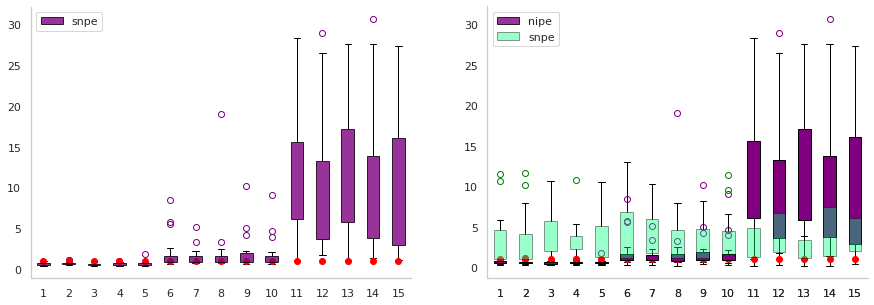
\includegraphics[width=1\linewidth]{images/box_plot_snpe_nipe_mdn.png}


% \caption{\label{box_plot_mdn}\textbf{Box plot for the variances of inferred and analytic posteriors - mdn used} \small The red points describe the ground truth from the analytic posterior. The green box plots show the distribution for the SNPE approach for every single parameter, while the purple box plots show the same for the NIPE approach. Here, we did not test NIPE-ONCE.}

% \end{figure}


\begin{figure}[h]
 \centering

        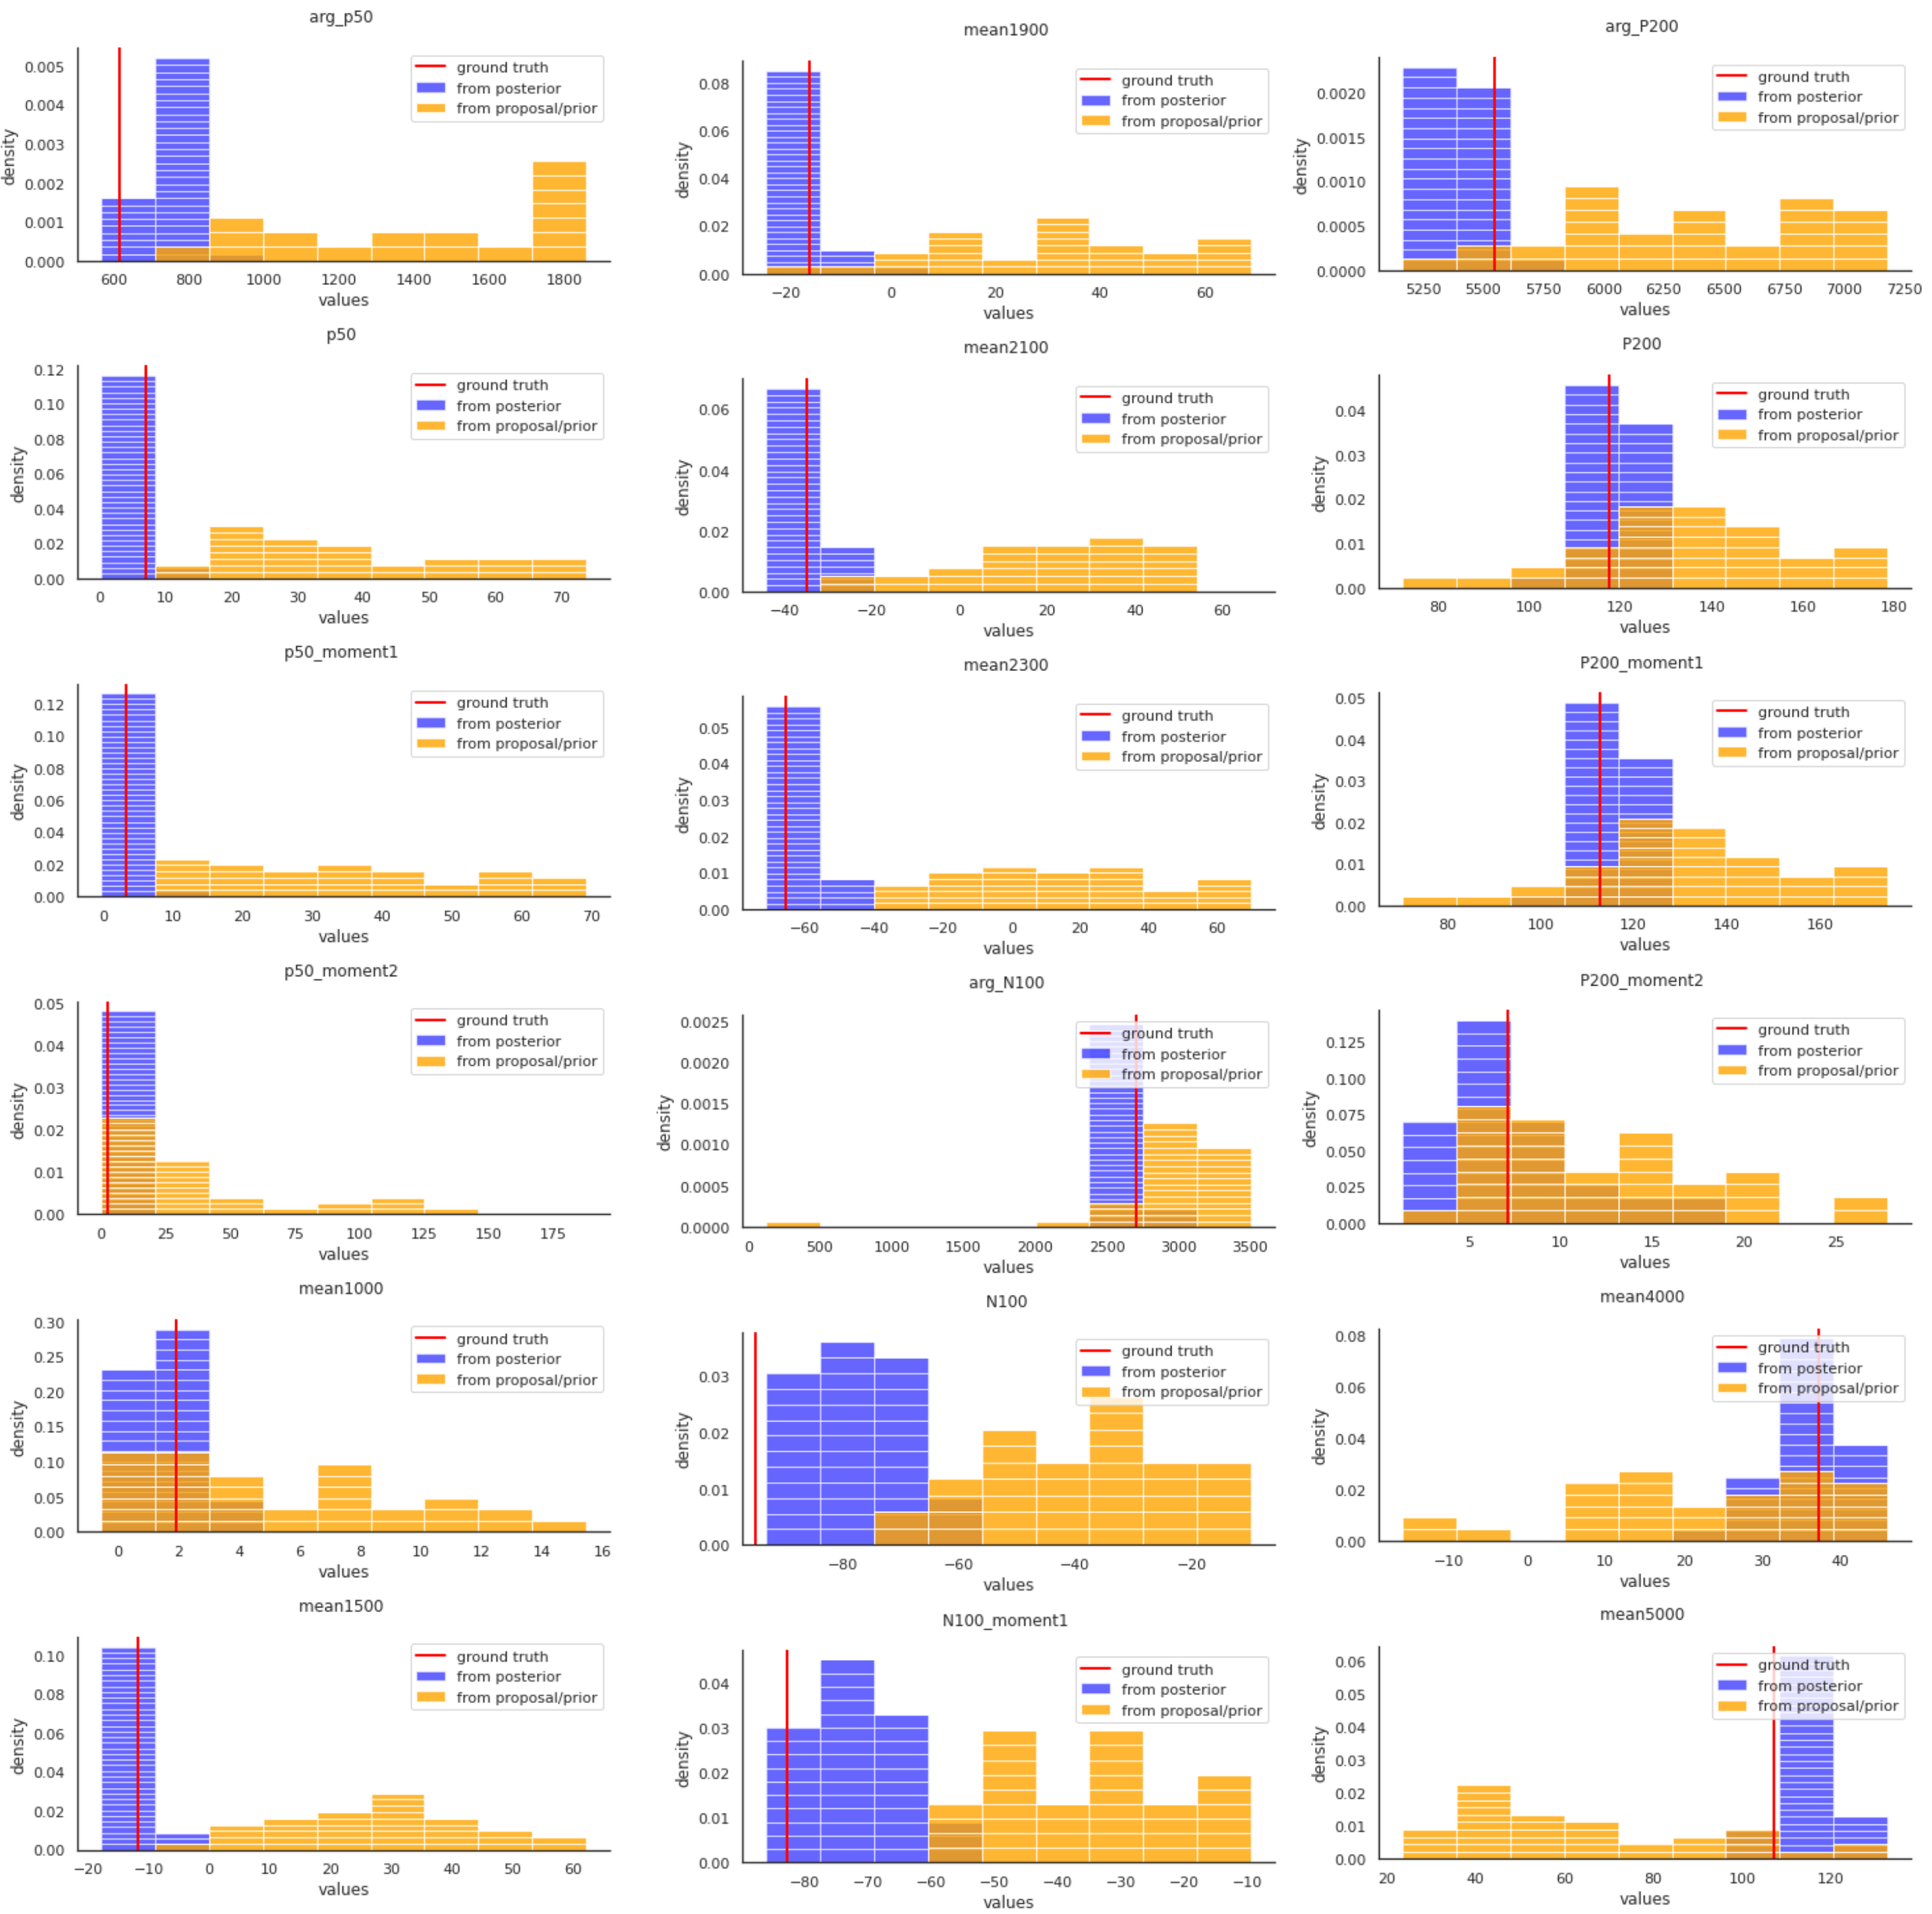
\includegraphics[width=0.99\linewidth]{images/all_histograms_appendix3.png}
        
        
\caption{\label{histo_appendix}\textbf{Histograms of the summary statistics.} \small All hand-crafted summary statistics are shown. The statistics derived from posterior simulations (blue) always include the ground truth value (shown in red). The statistics derived from the proposal (orange) have a broader distribution compared to the statistics from the posterior. The posterior was conditioned on a simulated observation here.}

\end{figure}

%  \begin{figure}
%  \centering


%         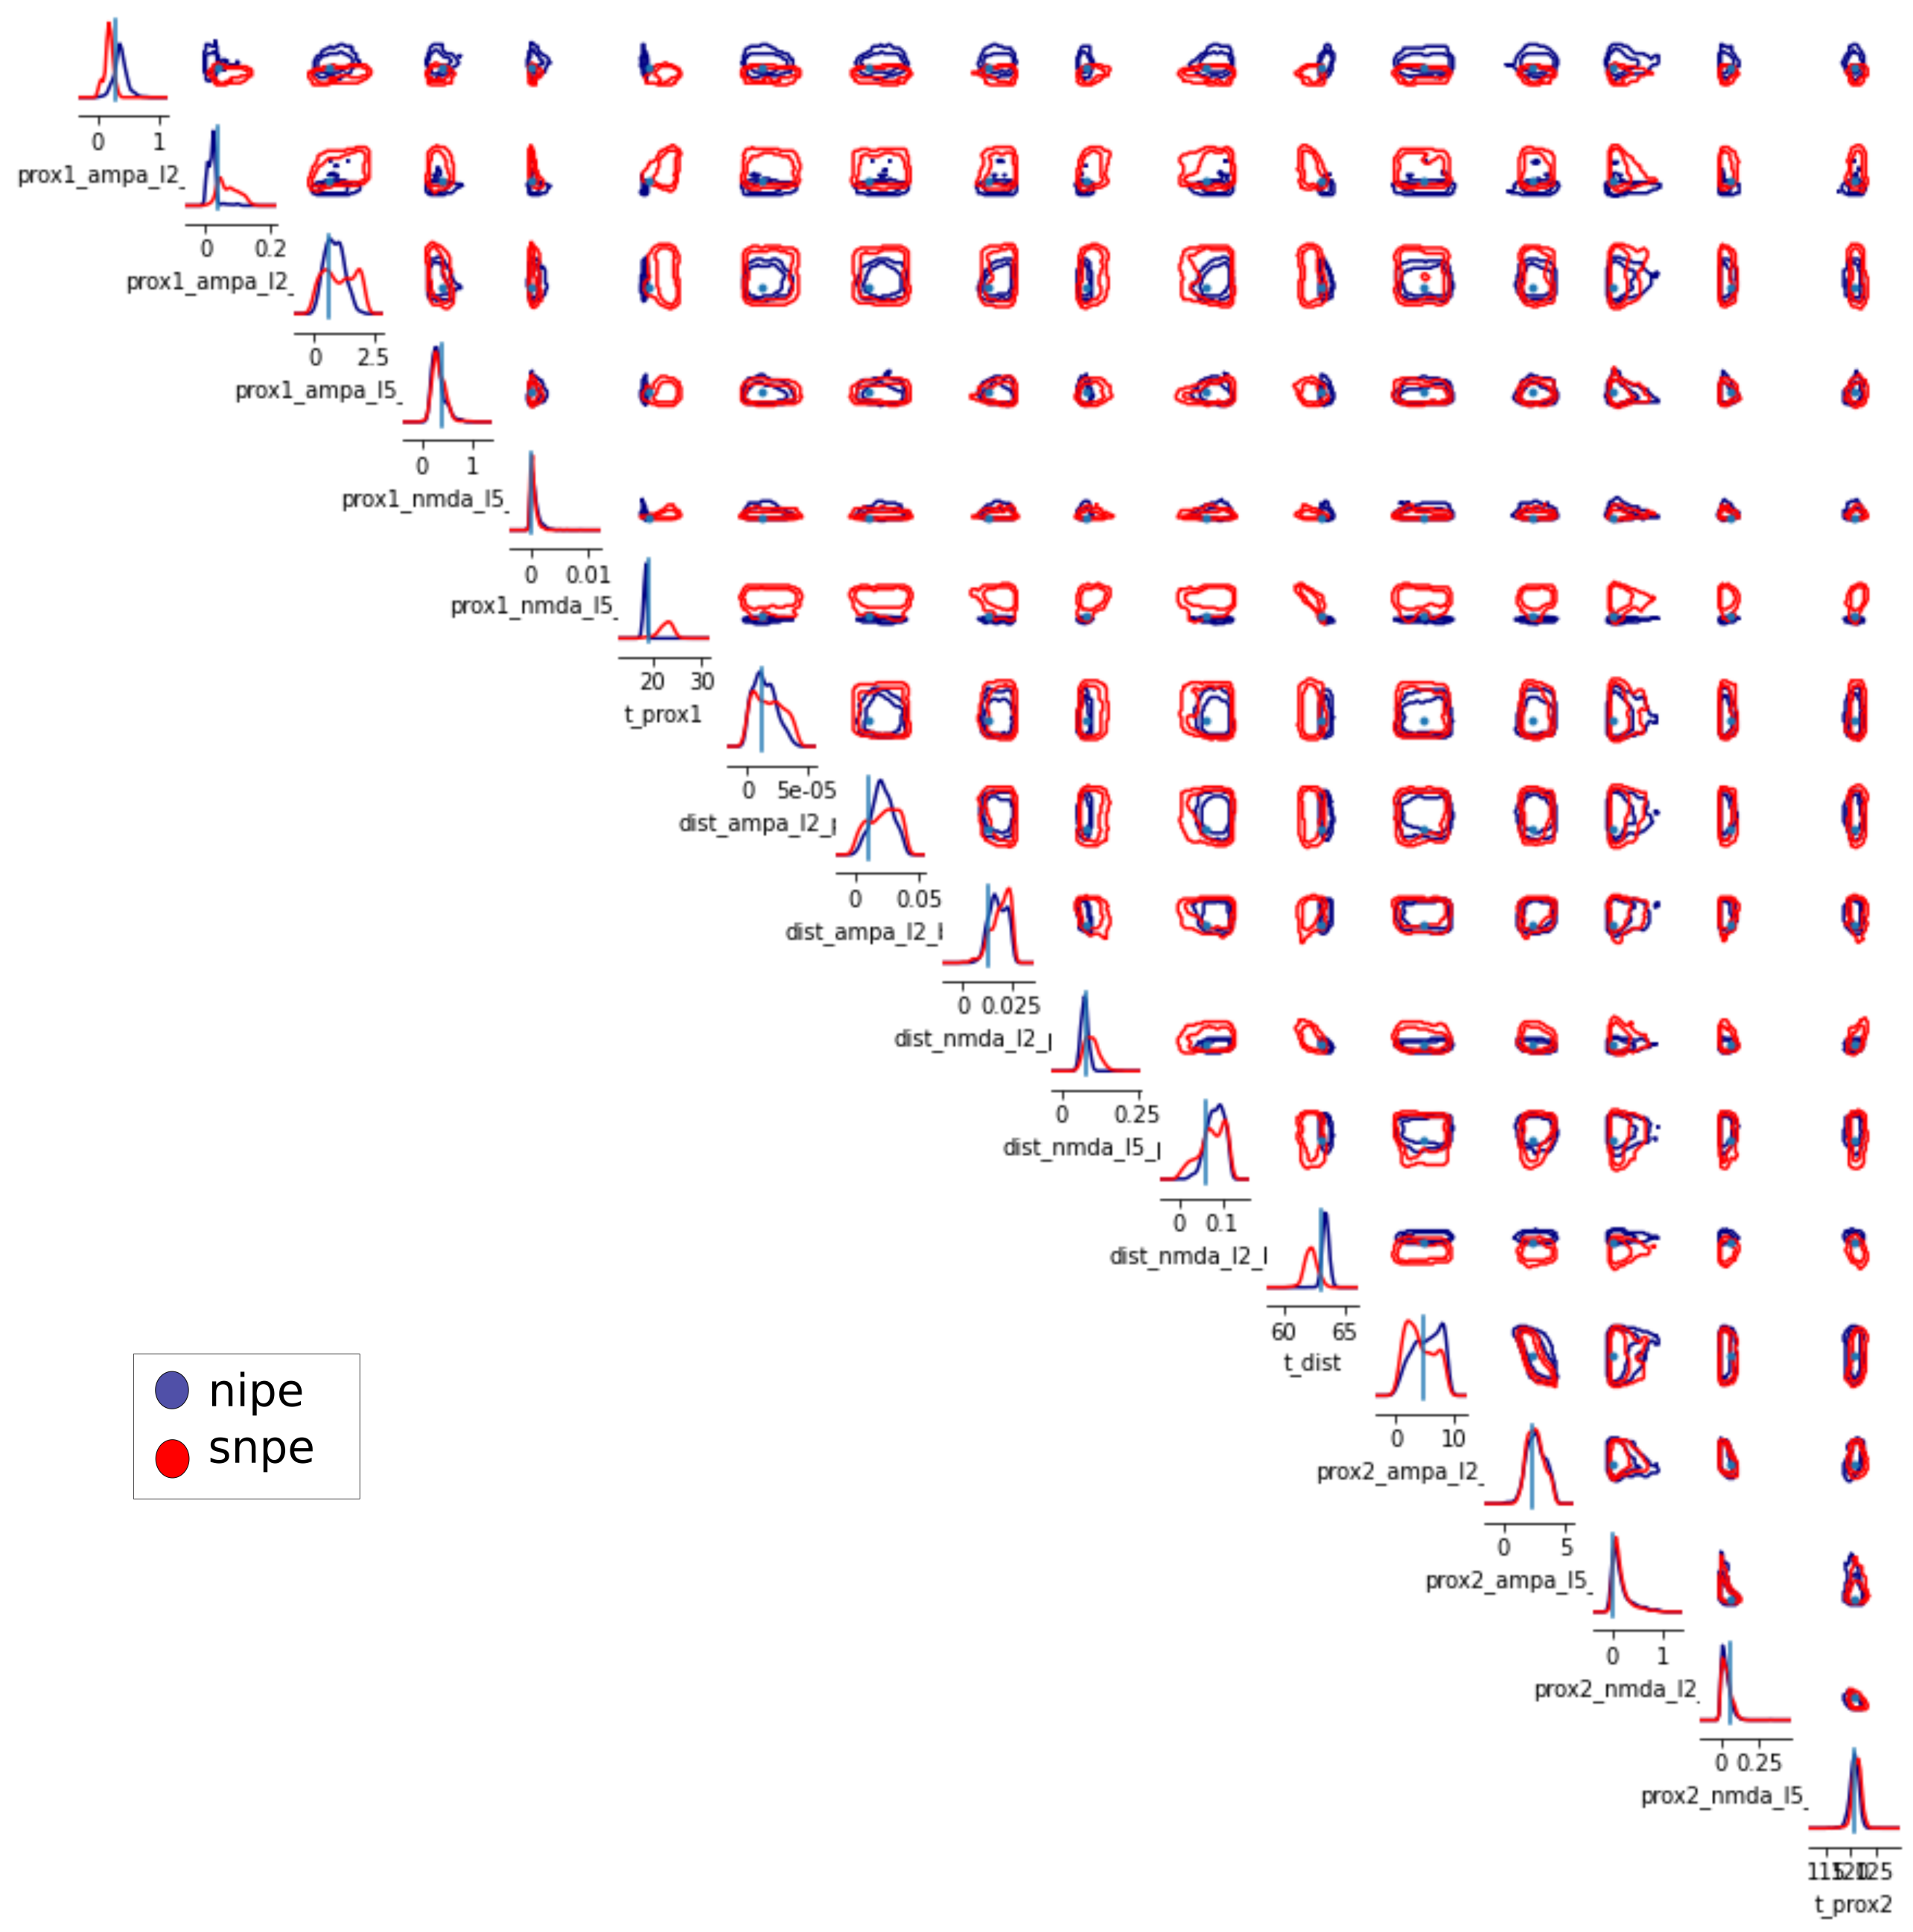
\includegraphics[width=0.90\linewidth]{images/contour_comp_snpe_nipe_label_reduced.png}


% \caption{\label{contour_nipe_snpe_appendix}\textbf{Contour density plots - comparsion between SNPE and NIPE} \small maf density estimator was used for both }

% \end{figure}

%  \begin{figure}
%  \centering


%         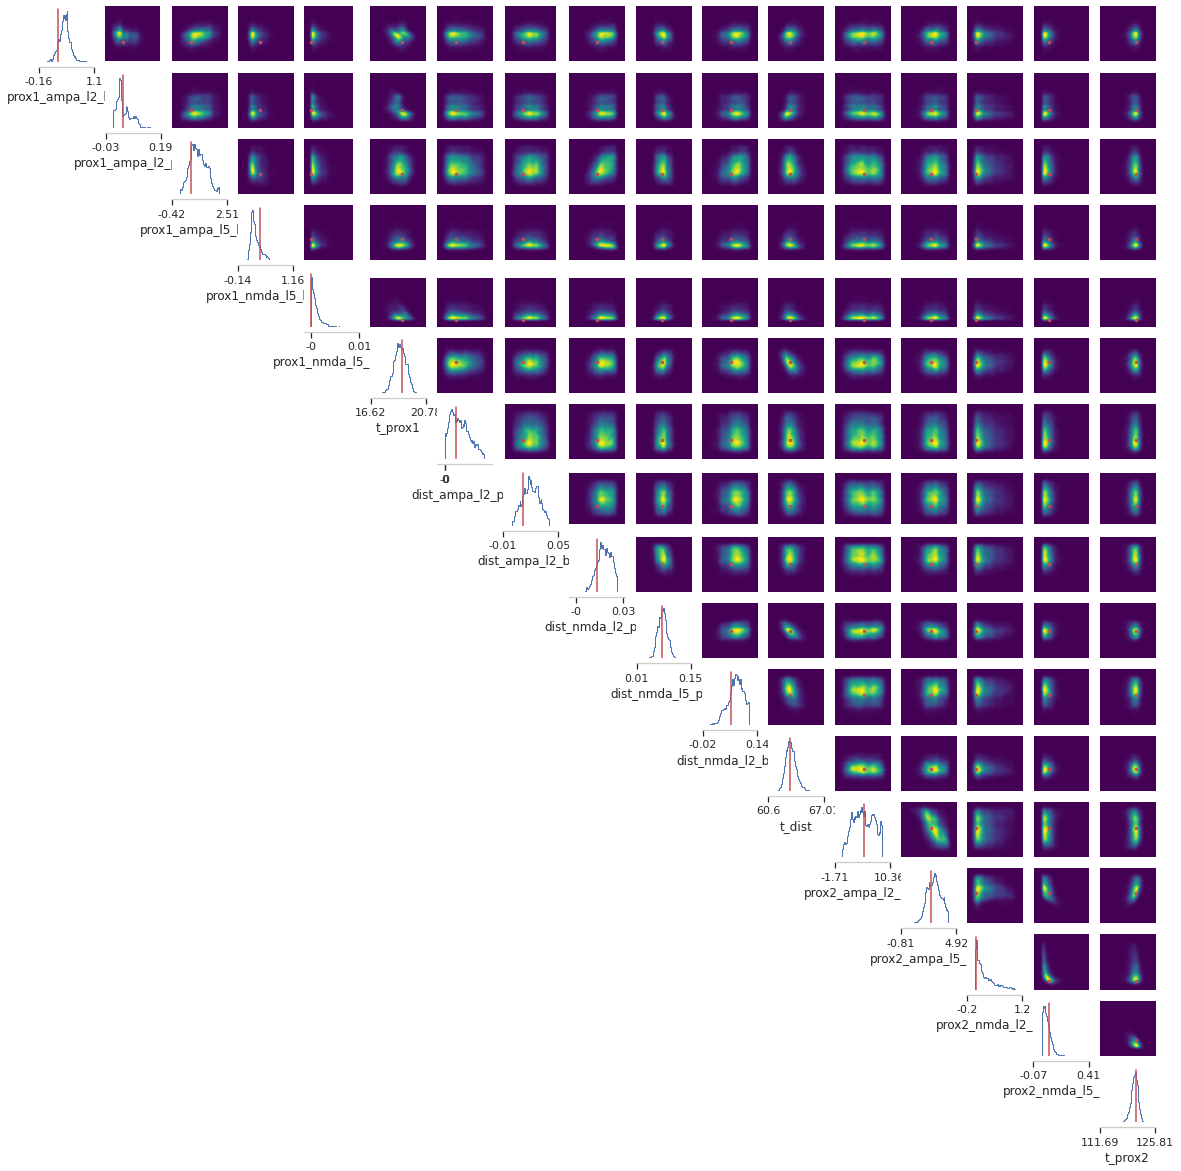
\includegraphics[width=0.90\linewidth]{images/kde_density_maf_ratio.png}
%         (a)
%         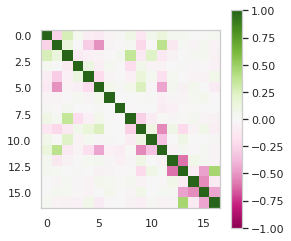
\includegraphics[width=0.4\linewidth]{images/correlation_matrix_maf_ratio.png}
%         (b)
%         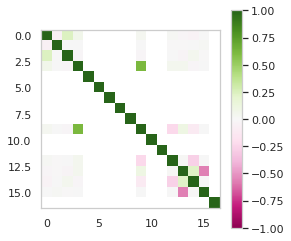
\includegraphics[width=0.4\linewidth]{images/cond_correlation_matrix_maf_ratio.png}
%         (c)
        

% \caption{\label{dens17nipe_app}\textbf{Density plots: NIPE + maf} \small inference on 17 parameters with the NIPE method, using a masked auto-regressive flow and a ratio for the number of simulations used per step such that there is a lower number of simulations for the first round and a higher number when doing inference on all parameters in the last round. (b) correlation matrix for the parameters. (c) conditional correlation matrix (all other parameters are fixes, except 2)}

% \end{figure}


%  \begin{figure}
%  \centering


%         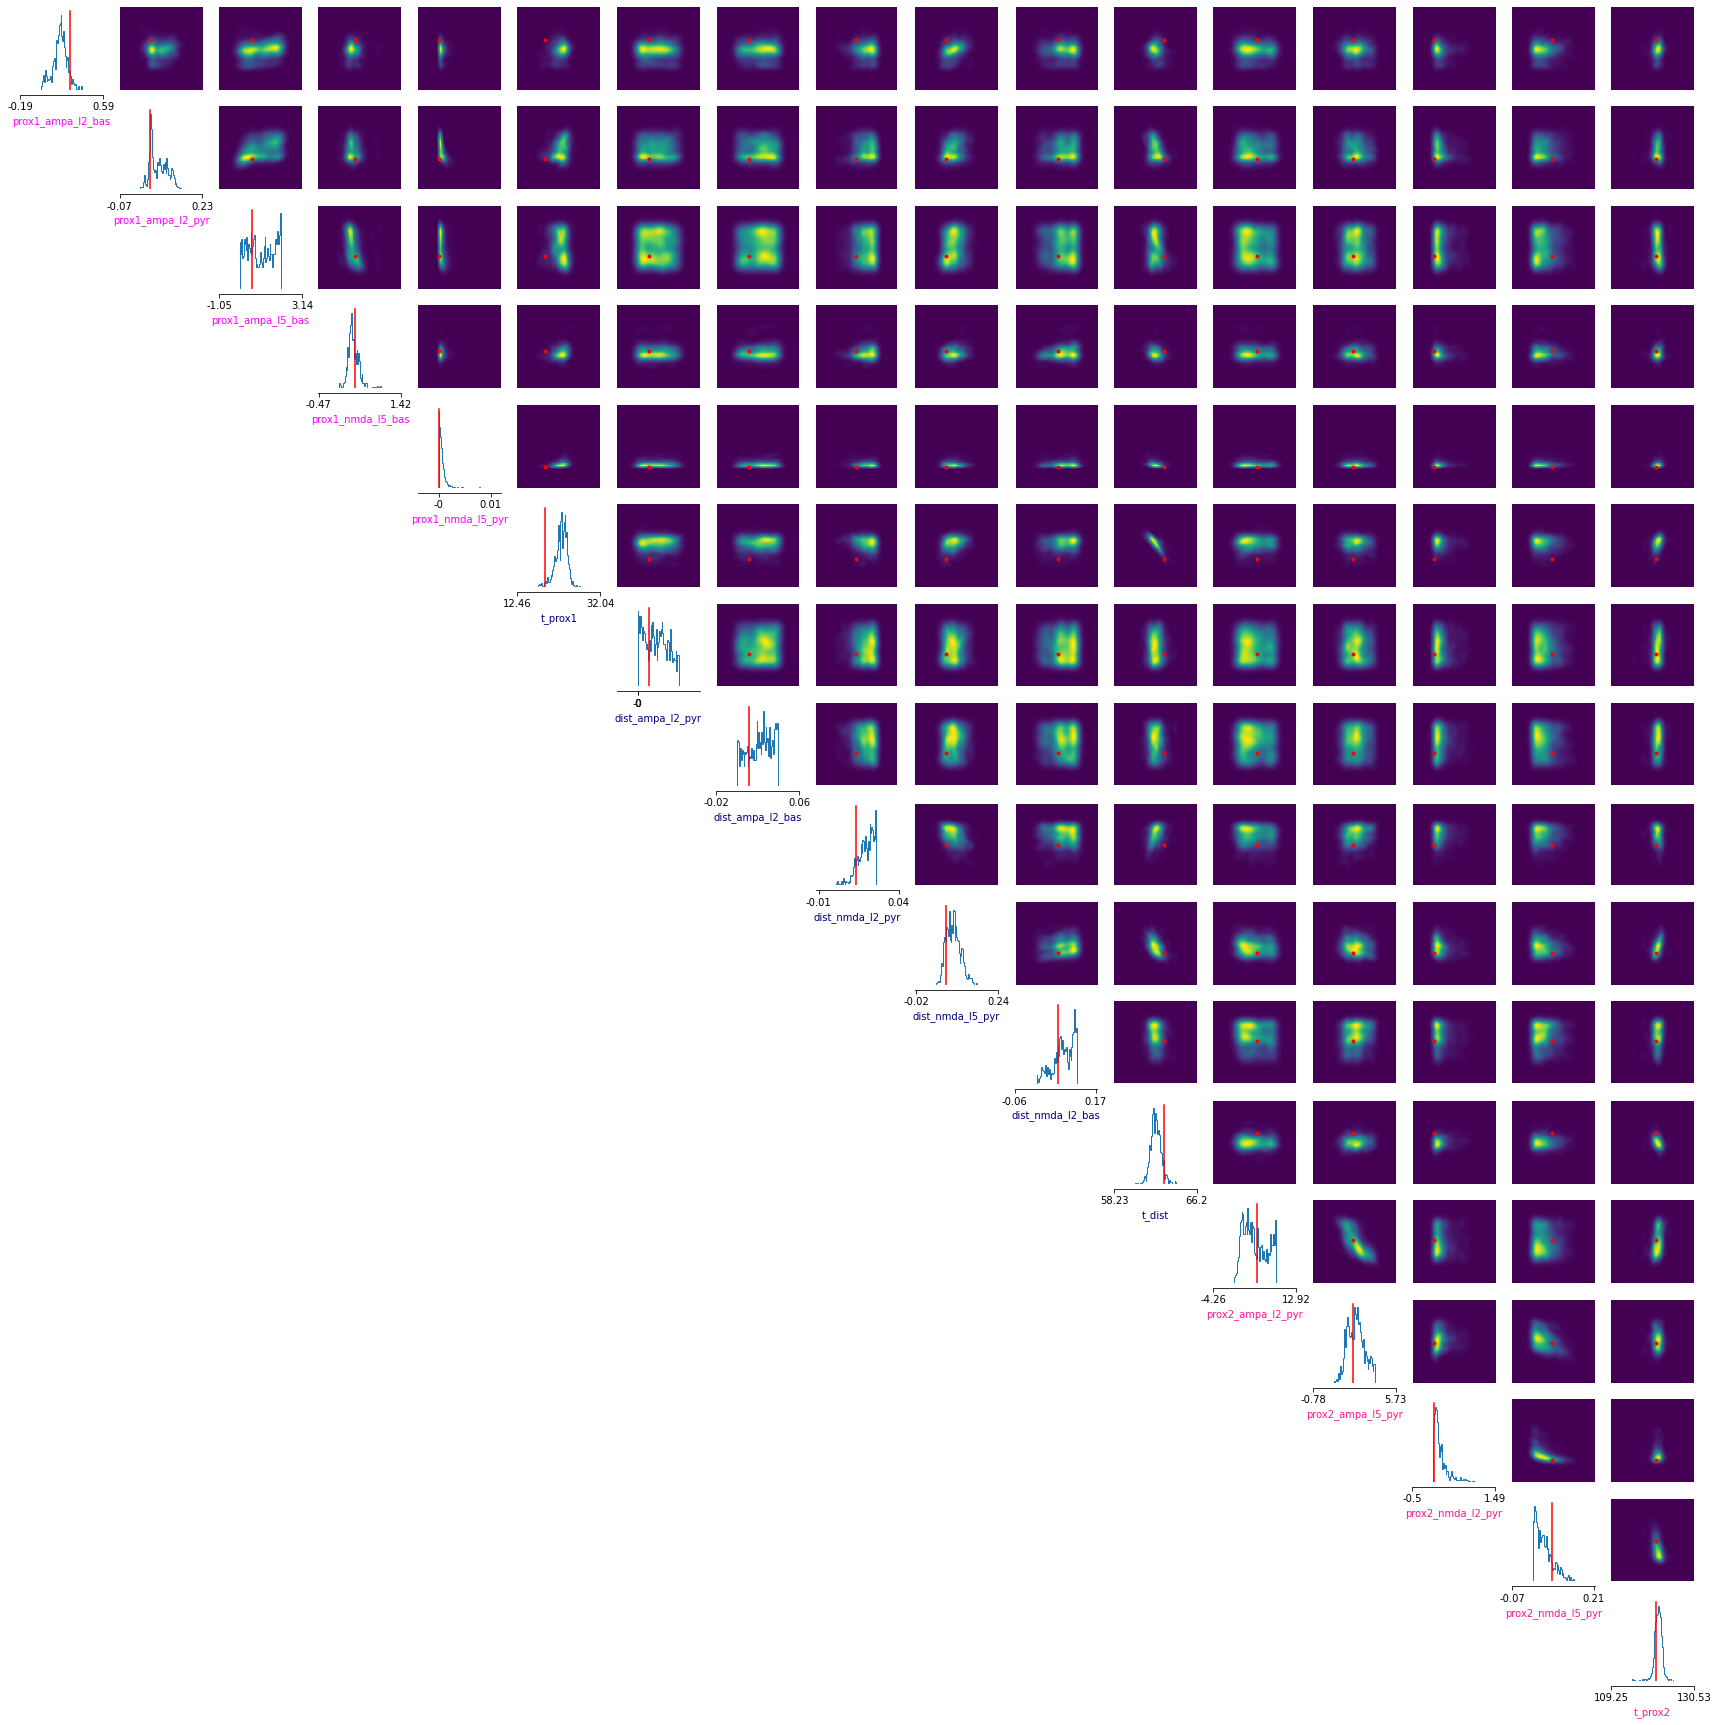
\includegraphics[width=0.90\linewidth]{images/kde_plot.png}
%         (a)
%         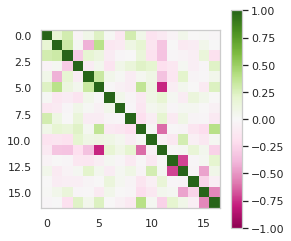
\includegraphics[width=0.4\linewidth]{images/correlation_matrix.png}
%         (b)
%         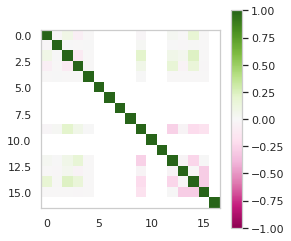
\includegraphics[width=0.4\linewidth]{images/cond_correlation_matrix_multi.png}
%         (c)

% \caption{\label{desn17_snpe_app}\textbf{Density plots: SNPE + maf} \small Inference on 17 parameters with the multi-round approach. (b) correlation matrix. (c) conditional correlation matrix  (all other parameters are fixes, except 2)}

% \end{figure}


 \begin{figure}[h]
 \centering


        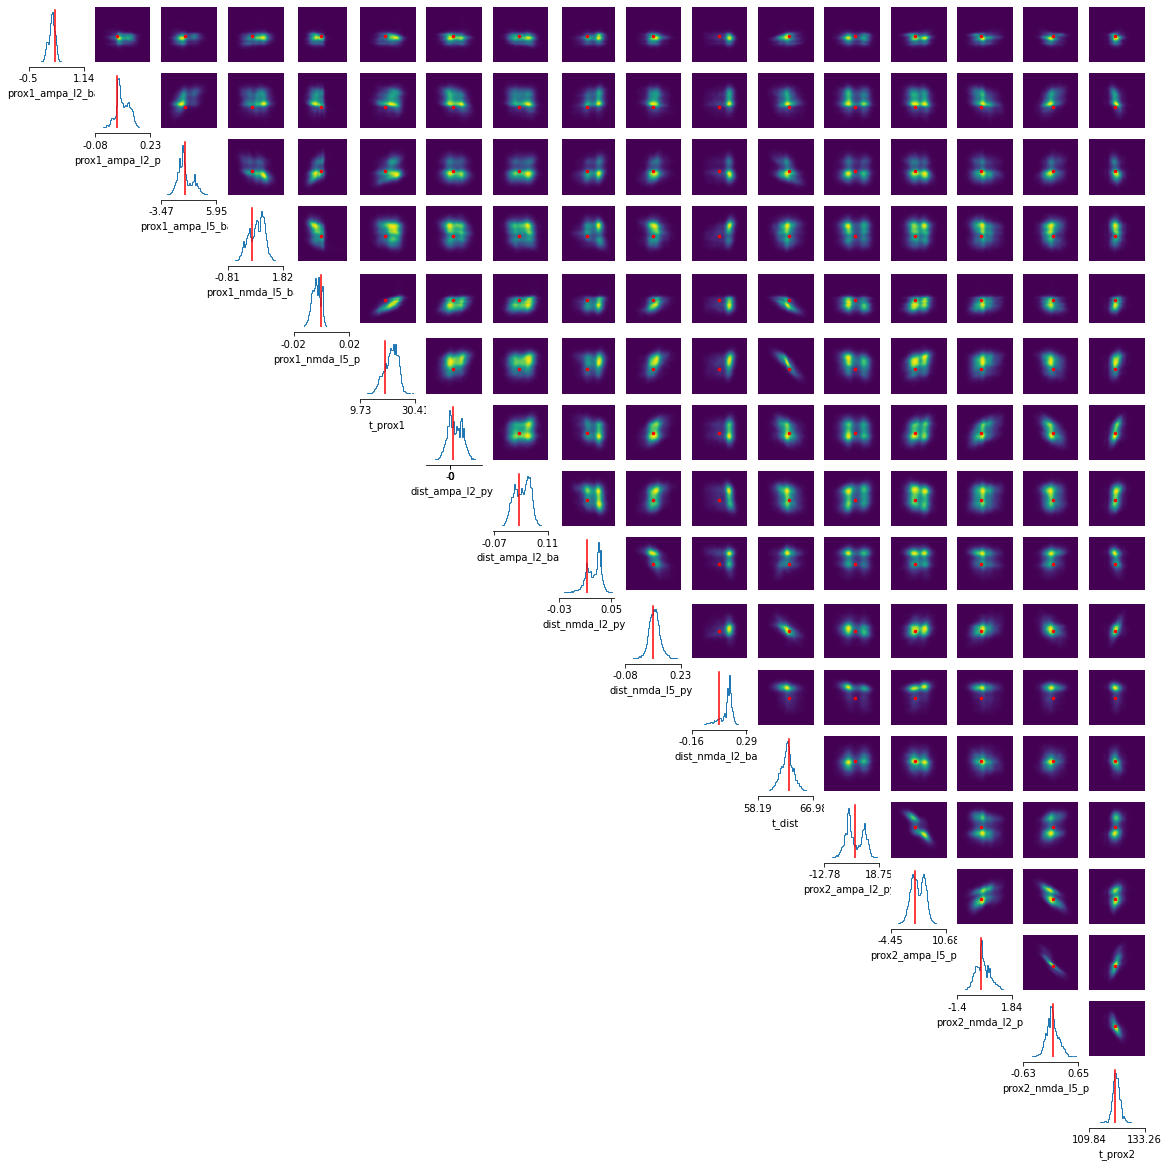
\includegraphics[width=0.90\linewidth]{images/thesis_fig6_6_leakage.png}
        %(a)
        %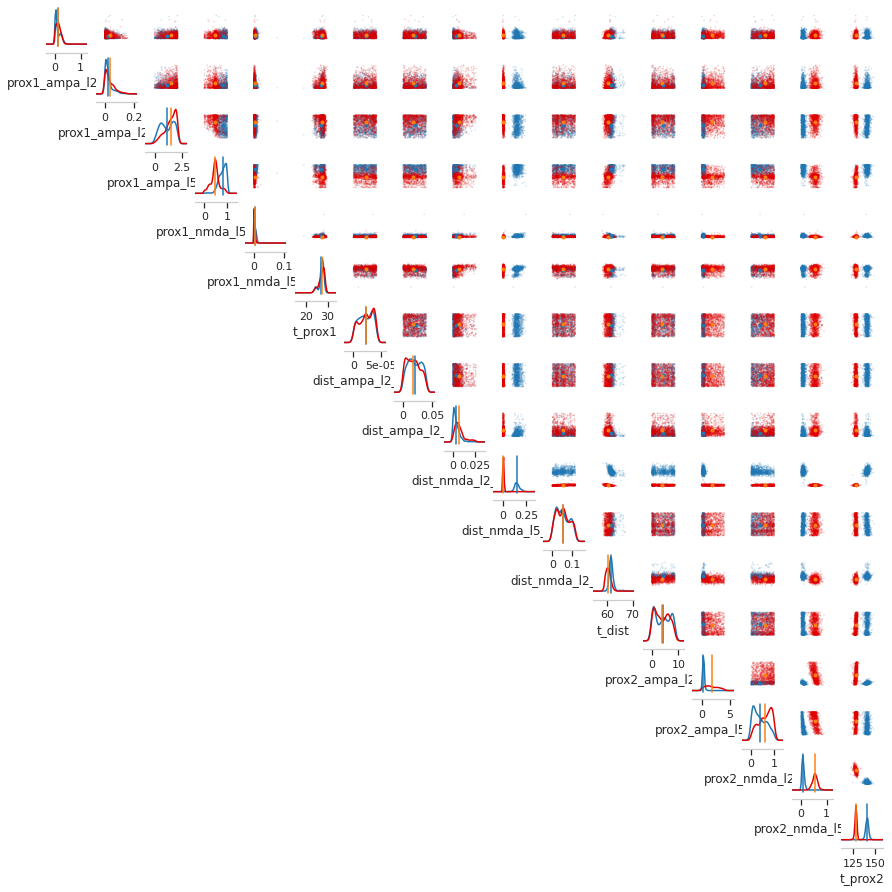
\includegraphics[width=0.45\linewidth]{images/scatter_density2.png}
        %(b)


\caption{\label{app_leakage}\textbf{Density plot for SNPE - leakage taken into account} \small Sampling from the posterior inferred by SNPE had an acceptance rate of only around $7e^{-5}$. Accepting all samples, also taking into account the ones not within the prior, revealed these 1D and 2D marginals. One can see that negative weights are seen as plausible by the inferred distribution. }

 \end{figure}
 
%   \begin{figure}
%  \centering


%         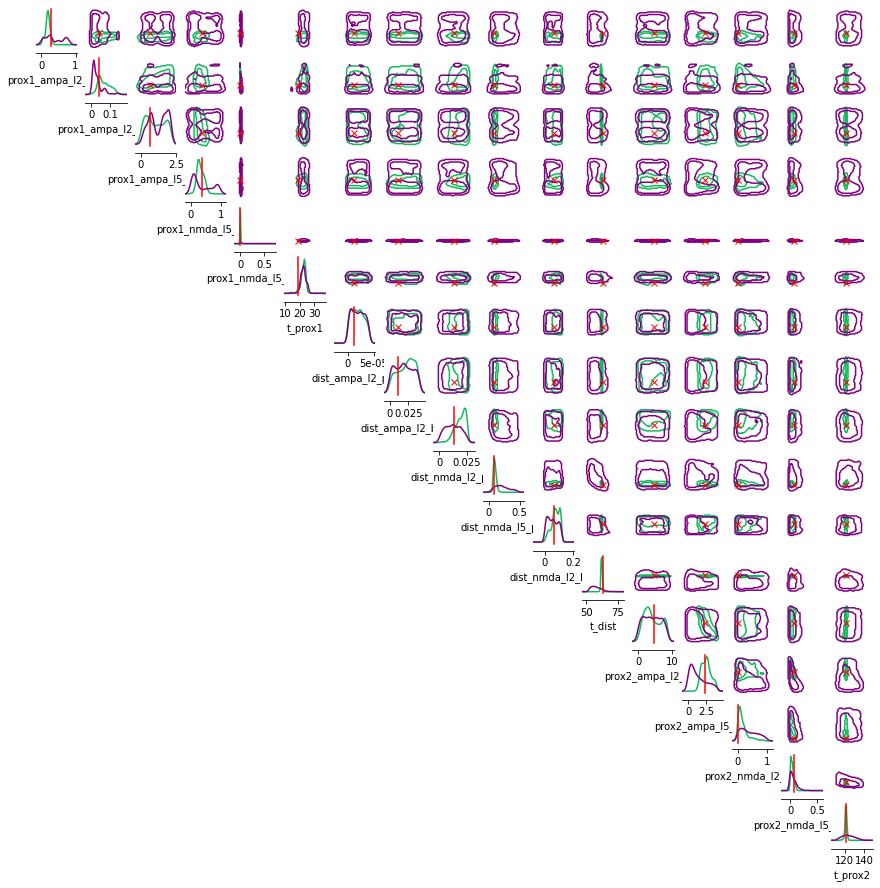
\includegraphics[width=0.99\linewidth]{images/contour_plot_snpe_nipe_once_restricted.png}


% \caption{\label{contour_nipe_snpe}\textbf{Contour density plots - comparison between SNPE and NIPE (once restricted)} \small A nsf density estimator was used for both. 68\% and 95\% percentiles of the posterior densities are shown as contour lines. True parameter values are plotted in red. The 1d marginals are on the diagonal, the 2d marginals off-diagonal.}

% \end{figure}



%   \begin{figure}
%  \centering


%         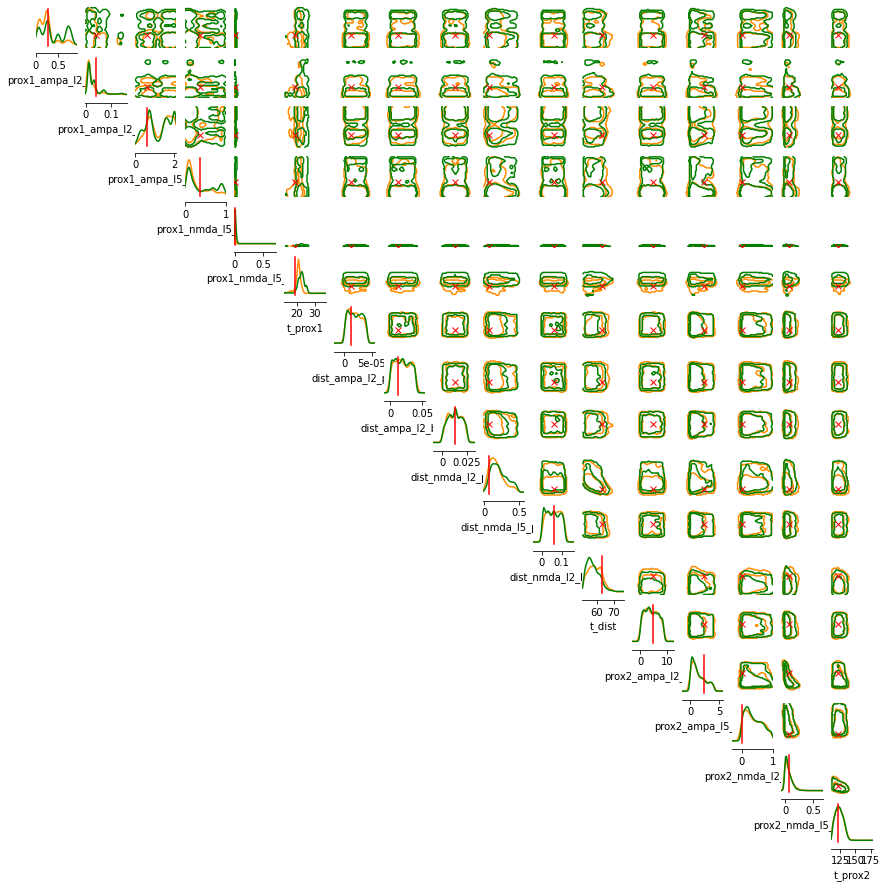
\includegraphics[width=0.99\linewidth]{images/contour_comp_once_green_normal_orange.png}


% \caption{\textbf{Contour density plots - comparison between NIPE (normal) and NIPE (once restricted)} \small A nsf density estimator was used for both. 68\% and 95\% percentiles of the posterior densities are shown as contour lines. True parameter values are plotted in red. The 1d marginals are on the diagonal, the 2d marginals off-diagonal. NIPE (normal) is plotted in orange, whereas NIPE (restricted once) is plotted in green.}

% \end{figure}

%  \begin{figure}
%  \centering


%         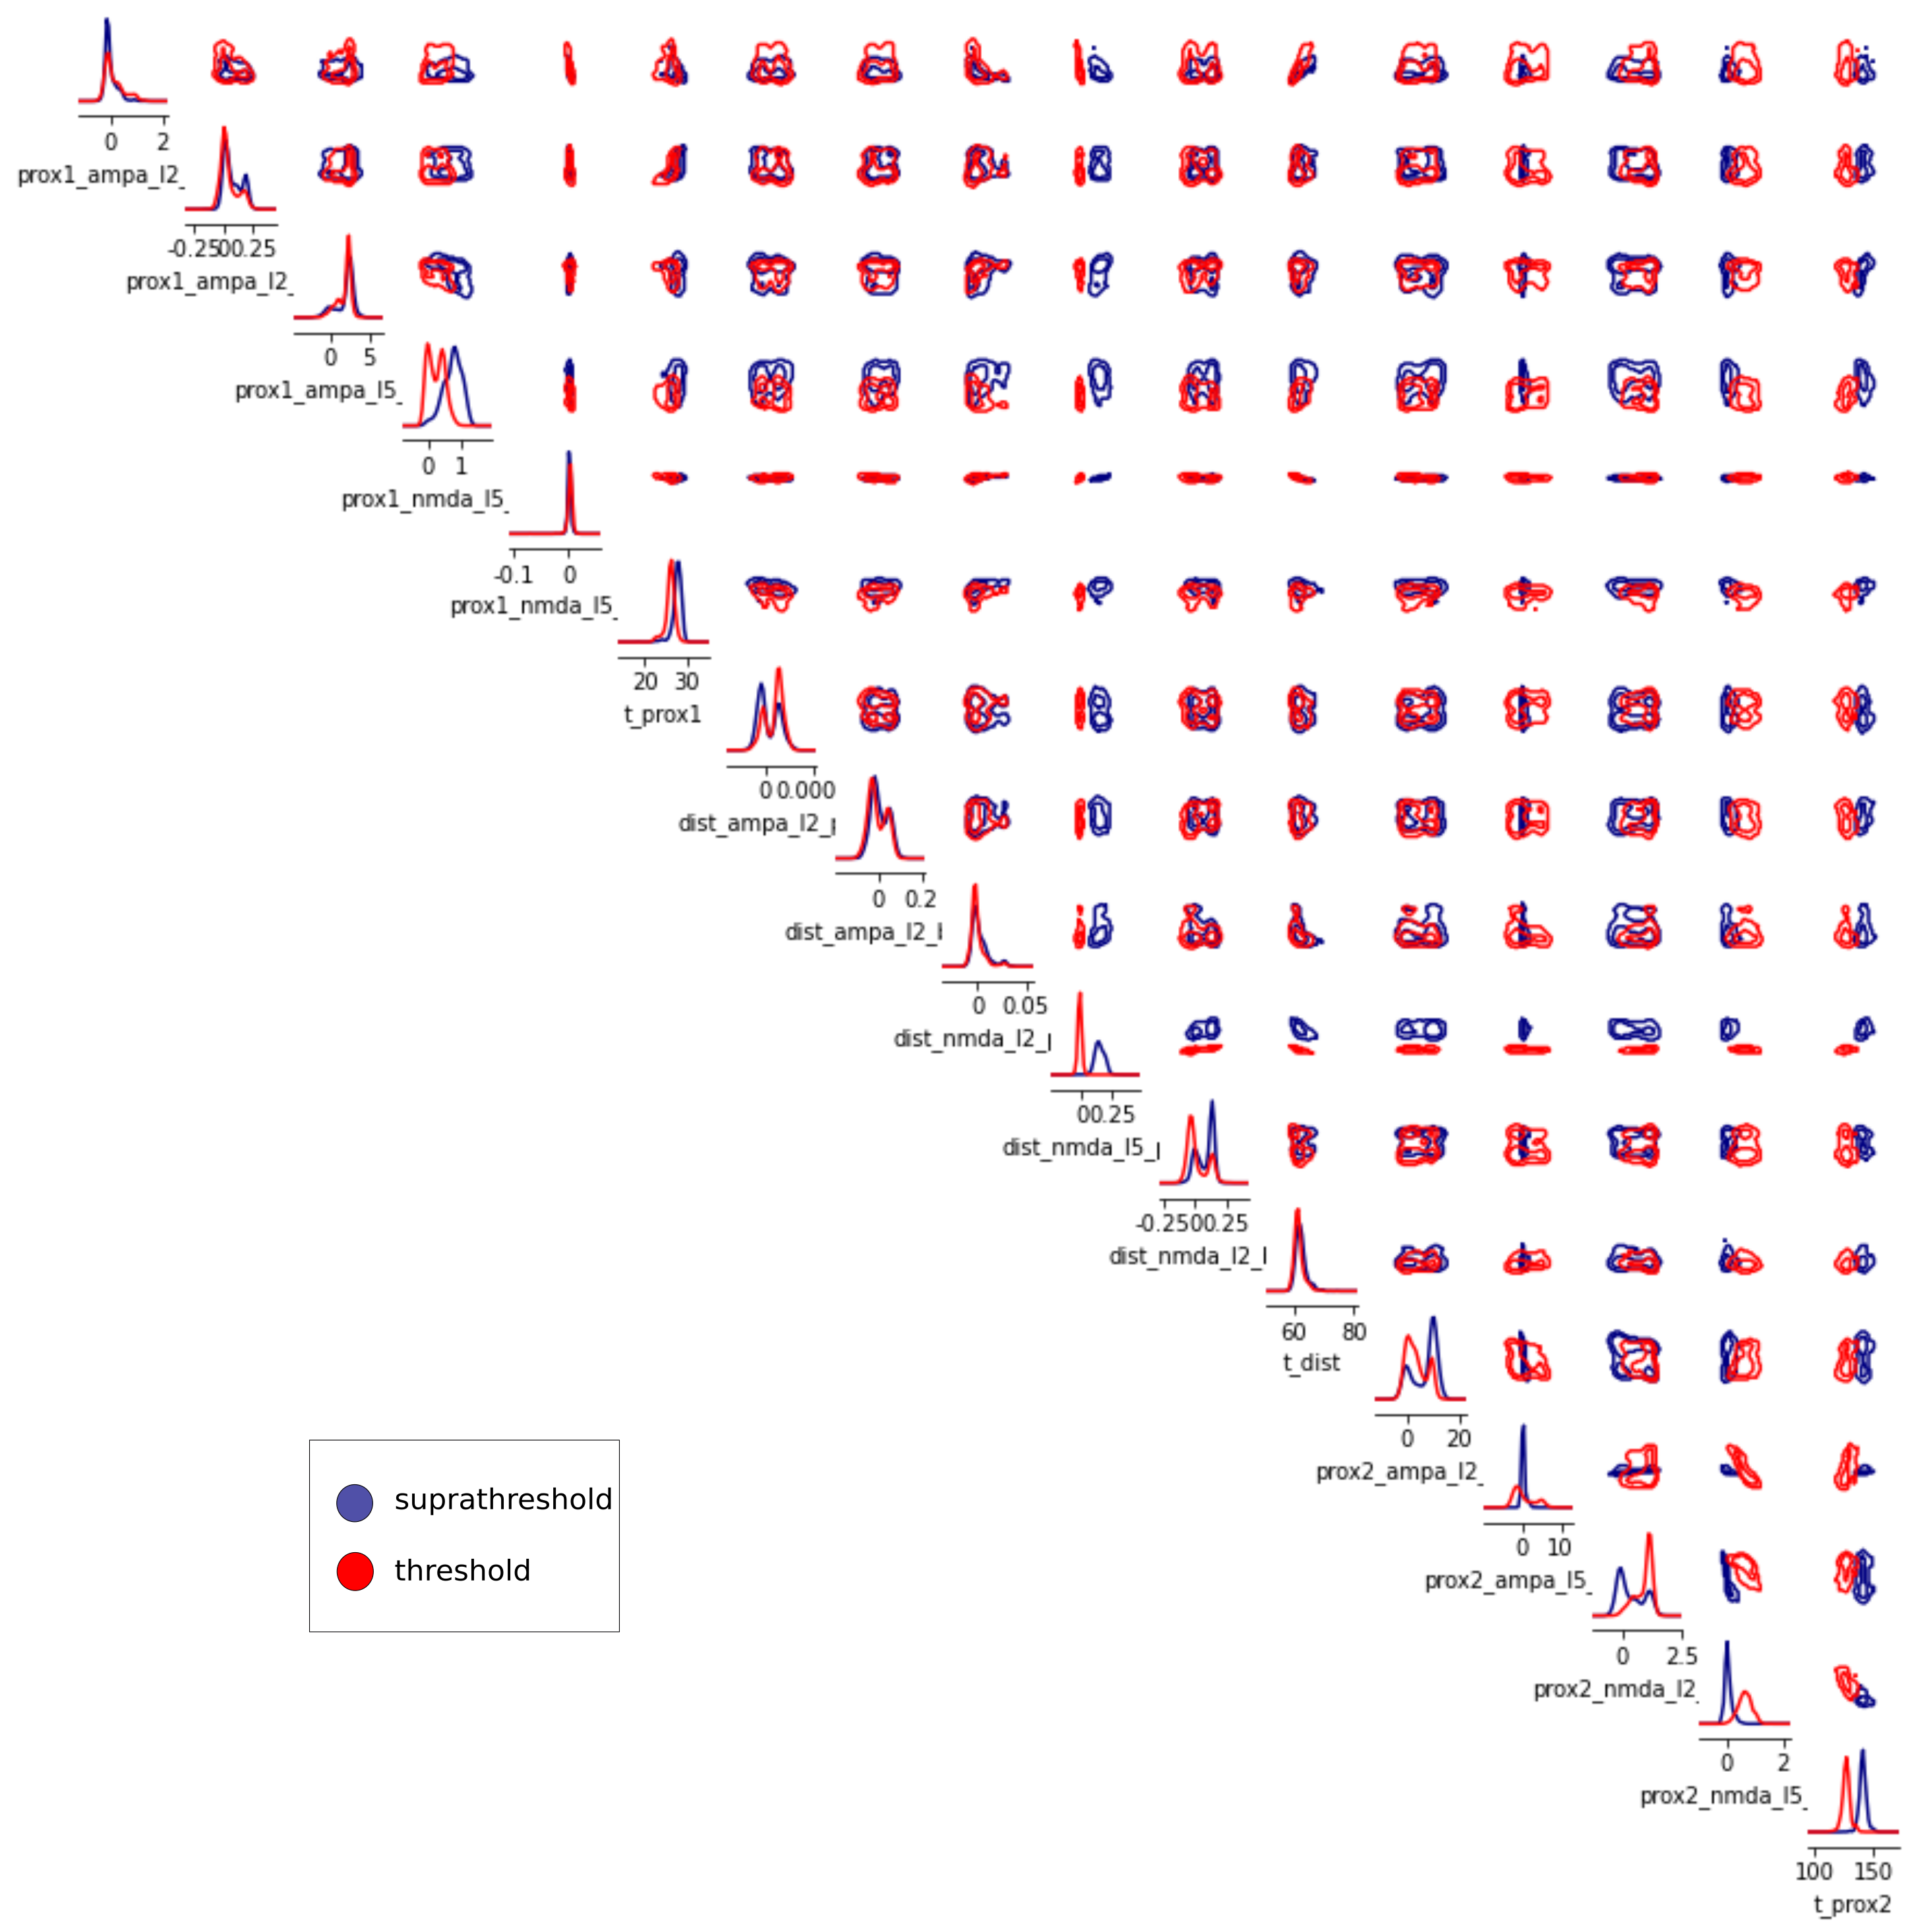
\includegraphics[width=0.99\linewidth]{images/contour_plot_posteriors_snpe_labels.png}
%         %(a)
%         %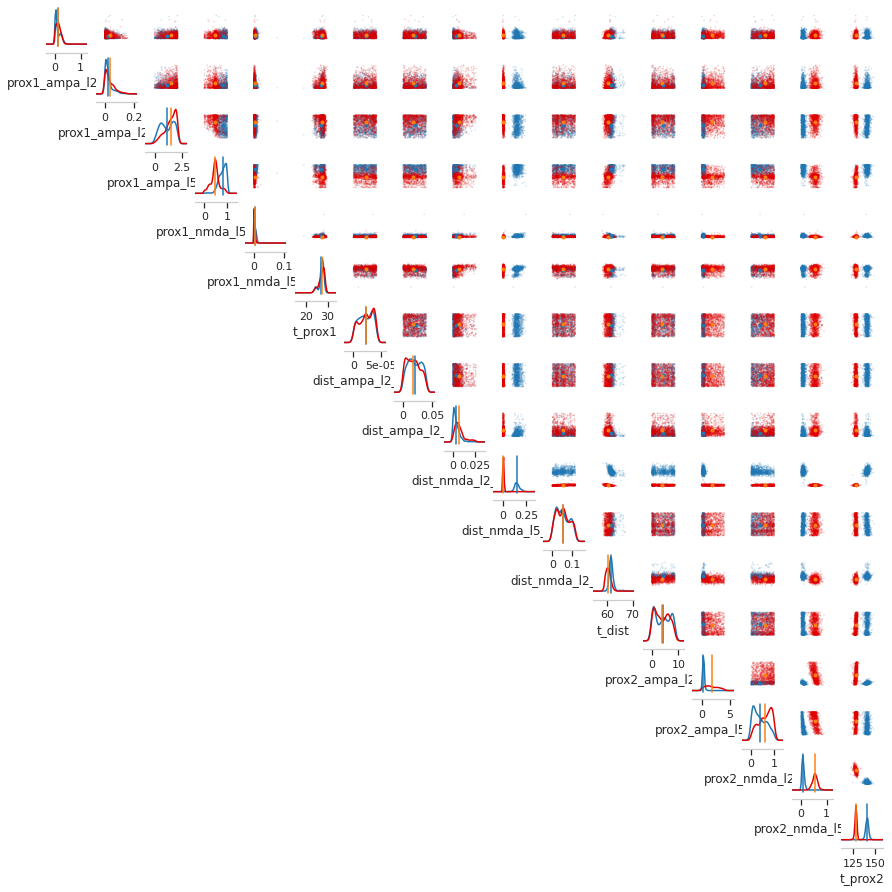
\includegraphics[width=0.45\linewidth]{images/scatter_density2.png}
%         %(b)


% \caption{\label{app_exp_contour}\textbf{Contour density plots- SNPE} \small Comparison of the threshold and the suprathreshold condition. Contour plots with 68\% percentile and 95\% percentile. In blue, the densities for the suprathreshold condition are visualized, whereas the densities for the threshold condition are visualized in red. On the diagonal, one can see the 1d marginals, and the 2d marginals are plotted off-diagonal.}

% %the parameter values that were found by \cite{jones2007neural}}

% \end{figure}





\end{document}
